\documentclass[10pt,a4paper]{article}
\usepackage{iftex}
\ifPDFTeX
  \usepackage[T1]{fontenc}\usepackage[utf8]{inputenc}\usepackage{lmodern}
\else
  \usepackage{fontspec}
\fi
\usepackage[french]{babel}
\usepackage[a4paper,margin=1.9cm,top=1.7cm,bottom=1.8cm]{geometry}
\usepackage{amsmath,amssymb}
\usepackage{booktabs,array}
\usepackage[table]{xcolor}
\usepackage{graphicx,float,caption}
\usepackage{fancyhdr,lastpage,titlesec,enumitem}
\usepackage{hyperref}
\definecolor{Forest}{HTML}{174F43}\definecolor{Muted}{HTML}{65756A}\definecolor{Sand}{HTML}{FBF1E3}
\hypersetup{colorlinks=true,linkcolor=Forest,urlcolor=Forest,pdftitle={SWI uniforme, fréquence de reconnaissance CatNat sécheresse et intervalles}}
\captionsetup{font={small,color=Muted},labelfont={bf,color=Forest},skip=3pt}
\setlength{\parindent}{0pt}\setlength{\parskip}{5pt}\linespread{1.06}
\titleformat{\section}{\Large\bfseries\color{Forest}}{\thesection}{.6em}{}
\titleformat{\subsection}{\normalsize\bfseries\color{Forest}}{}{0pt}{}
\pagestyle{fancy}\fancyhf{}\renewcommand{\headrulewidth}{0pt}
\fancyhead[L]{\small\bfseries\color{Forest}CLAIR / NOTE MÉTHODOLOGIQUE}
\fancyfoot[R]{\footnotesize\color{Forest}\thepage\,/\,\pageref{LastPage}}
\newcommand{\smallnote}[1]{{\small\color{Muted}#1}}
% Fichier généré par python -m pipeline.make_tables ; ne pas modifier à la main.
\newcommand{\metaTable}{%
34\,746 communes, 1989--2022, 1\,181\,364 lignes
}
\newcommand{\tabModels}{%
\begin{tabular}{lrrrrr}\toprule
Modèle & Log-loss & Gain & Brier & AUC & Attendu \\\midrule
Fréquence constante & 0{,}1542 & 0{,}0\,\% & 0{,}0339 & 0{,}448 & 25\,790 \\
Fréquence communale crédibilisée & 0{,}1455 & 5{,}6\,\% & 0{,}0328 & 0{,}702 & 25\,790 \\
GLM, SWI uniforme & 0{,}1353 & 12{,}2\,\% & 0{,}0325 & 0{,}778 & 27\,035 \\
GLM, SWI uniforme + exposition & 0{,}1218 & 21{,}0\,\% & 0{,}0308 & 0{,}854 & 26\,408 \\
GLM complet (+ historique publié) & 0{,}1210 & 21{,}5\,\% & 0{,}0311 & 0{,}862 & 29\,885 \\
Gradient boosting complet & 0{,}1253 & 18{,}8\,\% & 0{,}0296 & 0{,}841 & 24\,783 \\
GLM complet + aléa argile communal & 0{,}1151 & 25{,}4\,\% & 0{,}0303 & 0{,}884 & 29\,039 \\
Gradient boosting + aléa argile communal & 0{,}1213 & 21{,}4\,\% & 0{,}0293 & 0{,}864 & 24\,564 \\
\bottomrule\end{tabular}
}
\newcommand{\tabModelsRecent}{%
\begin{tabular}{lrrrr}\toprule
Modèle & Log-loss & Gain & AUC & Attendu \\\midrule
Fréquence constante & 0{,}2192 & 0{,}0\,\% & 0{,}552 & 11\,149 \\
Fréquence communale crédibilisée & 0{,}2110 & 3{,}7\,\% & 0{,}700 & 11\,149 \\
GLM, SWI uniforme & 0{,}1879 & 14{,}3\,\% & 0{,}796 & 12\,973 \\
GLM, SWI uniforme + exposition & 0{,}1730 & 21{,}1\,\% & 0{,}859 & 11\,623 \\
GLM complet (+ historique publié) & 0{,}1664 & 24{,}1\,\% & 0{,}867 & 12\,866 \\
Gradient boosting complet & 0{,}1770 & 19{,}3\,\% & 0{,}841 & 13\,218 \\
GLM complet + aléa argile communal & 0{,}1582 & 27{,}8\,\% & 0{,}892 & 12\,305 \\
Gradient boosting + aléa argile communal & 0{,}1686 & 23{,}1\,\% & 0{,}870 & 12\,761 \\
\bottomrule\end{tabular}
}
\newcommand{\tabByYear}{%
\begin{tabular}{rrrrrr}\toprule
Année & Observé & Crédibilité & GLM & Obs./att. & AUC \\\midrule
2005 & 1521 & 974 & 1\,716 & 0{,}89 & 0{,}902 \\
2006 & 323 & 918 & 1\,030 & 0{,}31 & 0{,}889 \\
2007 & 203 & 953 & 644 & 0{,}32 & 0{,}954 \\
2008 & 121 & 918 & 504 & 0{,}24 & 0{,}919 \\
2009 & 596 & 881 & 1\,299 & 0{,}46 & 0{,}869 \\
2010 & 100 & 843 & 634 & 0{,}16 & 0{,}910 \\
2011 & 2247 & 831 & 1\,965 & 1{,}14 & 0{,}900 \\
2012 & 648 & 798 & 557 & 1{,}16 & 0{,}955 \\
2013 & 23 & 861 & 138 & 0{,}17 & 0{,}964 \\
2014 & 44 & 852 & 451 & 0{,}10 & 0{,}964 \\
2015 & 205 & 819 & 1\,119 & 0{,}18 & 0{,}935 \\
2016 & 982 & 789 & 304 & 3{,}23 & 0{,}916 \\
2017 & 2104 & 767 & 1\,165 & 1{,}81 & 0{,}886 \\
2018 & 4061 & 775 & 616 & 6{,}59 & 0{,}791 \\
2019 & 2923 & 821 & 852 & 3{,}43 & 0{,}788 \\
2020 & 3520 & 929 & 894 & 3{,}94 & 0{,}804 \\
2021 & 355 & 993 & 511 & 0{,}69 & 0{,}880 \\
2022 & 6894 & 1\,072 & 3\,662 & 1{,}88 & 0{,}817 \\
\bottomrule\end{tabular}
}
\newcommand{\tabCoef}{%
\begin{tabular}{lrr}\toprule
Variable & Coefficient & Rapport de cotes (1 écart-type) \\\midrule
\texttt{swi\_jja\_z} & $-$0{,}386 & 0{,}680 \\
\texttt{swi\_son\_z} & $-$0{,}260 & 0{,}771 \\
\texttt{swi\_min\_z} & 0{,}135 & 1{,}145 \\
\texttt{swi\_jja\_z\_prev} & 0{,}020 & 1{,}020 \\
\texttt{rp\_max\_log} & 0{,}870 & 2{,}386 \\
\texttt{rga\_mid\_share} & 0{,}292 & 1{,}338 \\
\texttt{rga\_high\_share} & 0{,}553 & 1{,}739 \\
\texttt{rga\_missing} & $-$0{,}027 & 0{,}974 \\
\texttt{log\_population} & 0{,}534 & 1{,}706 \\
\texttt{hist\_count} & 0{,}248 & 1{,}282 \\
\bottomrule\end{tabular}
}
\newcommand{\tabForecastAll}{%
\begin{tabular}{lrrrrr}\toprule
Modèle & RMSE & MAE & Corrél. & RMSE nat. & Corrél. nat. \\\midrule
Persistance (SWI d’été précédent) & 0{,}189 & 0{,}147 & 0{,}508 & 0{,}137 & 0{,}04 \\
Climatologie de la maille & 0{,}151 & 0{,}124 & 0{,}682 & 0{,}114 & 0{,}19 \\
Régression ridge & 0{,}123 & 0{,}096 & 0{,}769 & 0{,}089 & 0{,}50 \\
Gradient boosting & 0{,}147 & 0{,}111 & 0{,}681 & 0{,}113 & 0{,}36 \\
Forêt aléatoire & 0{,}135 & 0{,}104 & 0{,}718 & 0{,}099 & 0{,}40 \\
\bottomrule\end{tabular}
}
\newcommand{\tabForecastDry}{%
\begin{tabular}{lrrrrr}\toprule
Modèle & RMSE & MAE & Corrél. & RMSE nat. & Corrél. nat. \\\midrule
Persistance (SWI d’été précédent) & 0{,}219 & 0{,}170 & 0{,}600 & 0{,}188 & 0{,}09 \\
Climatologie de la maille & 0{,}200 & 0{,}179 & 0{,}763 & 0{,}180 & 0{,}21 \\
Régression ridge & 0{,}114 & 0{,}092 & 0{,}810 & 0{,}089 & 0{,}29 \\
Gradient boosting & 0{,}139 & 0{,}105 & 0{,}725 & 0{,}112 & 0{,}17 \\
Forêt aléatoire & 0{,}132 & 0{,}106 & 0{,}775 & 0{,}109 & 0{,}32 \\
\bottomrule\end{tabular}
}
\newcommand{\tabVariogram}{%
\begin{tabular}{lrrrr}\toprule
Modèle & Pépite ($\times10^{-3}$) & Palier ($\times10^{-3}$) & Portée (km) & Erreur pond. ($\times10^{-3}$) \\\midrule
spherique & 0{,}53 & 6{,}62 & 237 & 0{,}154 \\
exponentiel & 0{,}00 & 7{,}52 & 292 & 0{,}310 \\
gaussien & 1{,}63 & 5{,}56 & 206 & 0{,}173 \\
\bottomrule\end{tabular}
}
\newcommand{\tabKriging}{%
\begin{tabular}{lrrrrr}\toprule
Validation & RMSE & MAE & Couverture 95\,\% & Écart-type erreur std. & Points \\\midrule
Blocs de 100 km & 0{,}0395 & 0{,}0278 & 96{,}7\,\% & 0{,}76 & 600 \\
Blocs de 25 km & 0{,}0232 & 0{,}0170 & 97{,}9\,\% & 0{,}68 & 287 \\
\bottomrule\end{tabular}
}
\newcommand{\tabCriterion}{%
\begin{tabular}{lrrrrr}\toprule
Période de retour & Les deux & Critère seul & Arrêté seul & Sensibilité & Précision \\\midrule
10 ans & 33\,175 & 579\,890 & 8\,382 & 79{,}8\,\% & 5{,}4\,\% \\
25 ans & 27\,828 & 347\,408 & 13\,729 & 67{,}0\,\% & 7{,}4\,\% \\
50 ans & 23\,682 & 255\,282 & 17\,875 & 57{,}0\,\% & 8{,}5\,\% \\
\bottomrule\end{tabular}
}
\newcommand{\tabSeverity}{%
\begin{tabular}{rrrr}\toprule
Année & Anomalie JJA moyenne & ln(période de retour) & Communes reconnues \\\midrule
\textbf{2026} & \textbf{$-$1{,}59} & \textbf{4{,}45} & estimation \\
2011 & $-$1{,}06 & 4{,}08 & 2\,247 \\
2022 & $-$1{,}54 & 3{,}81 & 6\,894 \\
1989 & $-$1{,}45 & 3{,}36 & 3\,775 \\
1990 & $-$1{,}04 & 3{,}34 & 462 \\
1997 & $-$0{,}05 & 3{,}32 & 351 \\
2003 & $-$1{,}35 & 3{,}31 & 4\,352 \\
\bottomrule\end{tabular}
}
\newcommand{\tabRegionsNow}{%
\begin{tabular}{lrr}\toprule
Région & Part attendue & Communes attendues \\\midrule
Centre-Val de Loire & 36{,}6\,\% & 642 \\
Île-de-France & 35{,}7\,\% & 453 \\
Occitanie & 33{,}9\,\% & 1\,509 \\
Nouvelle-Aquitaine & 30{,}8\,\% & 1\,324 \\
Bourgogne-Franche-Comté & 30{,}8\,\% & 1\,135 \\
Grand Est & 23{,}6\,\% & 1\,205 \\
Auvergne-Rhône-Alpes & 22{,}3\,\% & 897 \\
Provence-Alpes-Côte d'Azur & 16{,}3\,\% & 155 \\
\bottomrule\end{tabular}
}
\newcommand{\nowcastSummary}{%
7\,870 communes attendues ; fourchette empirique 1\,040--18\,204
}
\newcommand{\tabDept}{%
\begin{tabular}{rrrr}\toprule
Département & Observé & Attendu & Rapport \\\midrule
58 & 560 & 105 & 5{,}31 \\
71 & 1003 & 252 & 3{,}99 \\
89 & 511 & 130 & 3{,}92 \\
39 & 752 & 212 & 3{,}55 \\
21 & 557 & 206 & 2{,}71 \\
18 & 624 & 257 & 2{,}43 \\
57 & 1206 & 504 & 2{,}39 \\
52 & 226 & 97 & 2{,}34 \\
\bottomrule\end{tabular}
}
\newcommand{\tabLag}{%
\begin{tabular}{rrrrr}\toprule
Année d’événement & Arrêtés & Médiane & 99\,\% & Maximum \\\midrule
2000 & 118 & 2{,}08 & 7{,}28 & 7{,}28 \\
2005 & 3233 & 2{,}55 & 3{,}80 & 6{,}38 \\
2010 & 104 & 0{,}81 & 1{,}51 & 1{,}70 \\
2015 & 205 & 1{,}07 & 1{,}74 & 2{,}14 \\
2018 & 4093 & 0{,}46 & 1{,}54 & 3{,}06 \\
2020 & 3734 & 0{,}63 & 1{,}72 & 2{,}47 \\
2022 & 7935 & 0{,}57 & 1{,}64 & 2{,}31 \\
\bottomrule\end{tabular}
}
\newcommand{\tabIntervals}{%
\begin{tabular}{lr}\toprule
Résultat 2026 & Valeur \\\midrule
Nombre attendu de communes reconnues & 7\,870 \\
Intervalle à 90\,\% de l'estimation (bootstrap par années) & 5\,462--9\,690 \\
Intervalle de prédiction à 80\,\% (backtest) & 1\,040--18\,204 \\
Intervalle de prédiction à 90\,\% (backtest) & 722--22\,409 \\
Couverture une année laissée de côté (28 ans), 80\,\% / 90\,\% & 79\,\% / 82\,\% \\
\bottomrule\end{tabular}
}
\newcommand{\tabOldScore}{%
\begin{tabular}{lrr}\toprule
Indicateur & Spearman & Intervalle à 90\,\% \\\midrule
Score composite d’origine & 0{,}28 & 0{,}13--0{,}42 \\
Aléa argile BRGM seul & 0{,}59 & 0{,}48--0{,}68 \\
Part de jours secs seule & $-$0{,}21 & $-$0{,}35--$-$0{,}07 \\
Modèle de fréquence & 0{,}49 & 0{,}35--0{,}63 \\
\bottomrule\end{tabular}
}
\newcommand{\tabClimateDecades}{%
\begin{tabular}{lrr}\toprule
Décennie & Années & Mailles sous le décile de 1959--1988 \\\midrule
1960s & 10 & 10{,}7\,\% \\
1970s & 10 & 12{,}1\,\% \\
1980s & 10 & 12{,}4\,\% \\
1990s & 10 & 29{,}0\,\% \\
2000s & 10 & 35{,}2\,\% \\
2010s & 10 & 34{,}1\,\% \\
2020s & 7 & 57{,}4\,\% \\
\bottomrule\end{tabular}
}
\newcommand{\climateTrend}{%
$-$0{,}021 par décennie (intervalle à 90\,\% : $-$0{,}034 à $-$0{,}007 ; Mann--Kendall $p=0{,}004$)
}
\newcommand{\tabSensitivity}{%
\begin{tabular}{rrrrr}\toprule
Année de base & Déplacement du SWI & En écarts-types & Communes attendues & Observé \\\midrule
2018 & 0{,}05 & 0{,}46 & 338 & 4061 \\
2018 & 0{,}00 & 0{,}00 & 629 & 4061 \\
2018 & $-$0{,}03 & $-$0{,}27 & 895 & 4061 \\
2018 & $-$0{,}06 & $-$0{,}55 & 1\,219 & 4061 \\
2018 & $-$0{,}10 & $-$0{,}91 & 1\,724 & 4061 \\
2022 & 0{,}05 & 0{,}46 & 1\,414 & 6894 \\
2022 & 0{,}00 & 0{,}00 & 3\,299 & 6894 \\
2022 & $-$0{,}03 & $-$0{,}27 & 4\,845 & 6894 \\
2022 & $-$0{,}06 & $-$0{,}55 & 5\,675 & 6894 \\
2022 & $-$0{,}10 & $-$0{,}91 & 6\,323 & 6894 \\
\bottomrule\end{tabular}
}
\newcommand{\geoMoran}{%
0{,}87 (p = 0{,}005, 8981 mailles, été 2022)
}
\newcommand{\geoBest}{%
spherique (portée 237\,km)
}
\newcommand{\tabInterp}{%
\begin{tabular}{lrrrr}\toprule
Méthode & RMSE & MAE & Biais & Couverture 95\,\% \\\midrule
Maille la plus proche & 0{,}0562 & 0{,}0319 & 0{,}0046 & -- \\
Pondération inverse (IDW) & 0{,}0373 & 0{,}0229 & 0{,}0025 & -- \\
Krigeage ordinaire & 0{,}0359 & 0{,}0218 & 0{,}0020 & 95{,}7\,\% \\
\bottomrule\end{tabular}
}
\newcommand{\tabInterpModel}{%
\begin{tabular}{lrr}\toprule
Source du SWI (GLM complet, 1995--2022) & Gain de log-loss & AUC \\\midrule
Maille la plus proche & 21{,}25\,\% & 0{,}8606 \\
SWI krigé au centre des communes & 21{,}53\,\% & 0{,}8620 \\
\bottomrule\end{tabular}
}
\newcommand{\interpSummary}{%
variogramme exponentiel standardisé (pépite 2{,}1\,\%) ; centre de commune à 3{,}2\,km de la maille la plus proche en médiane (4{,}8\,km au 95$^e$ centile) ; 898 mailles retirées, 68 étés
}

\graphicspath{{../../reports/figures/}}
\begin{document}
{\small\color{Muted}\textbf{NOTE 03}\quad SÉCHERESSE CATNAT}\vspace{4mm}

{\fontsize{25}{29}\selectfont\bfseries\color{Forest}Du SWI uniforme à une fréquence\par de reconnaissance avec intervalle.}\vspace{2mm}

{\large Prévision et géostatistique du SWI, modèle de fréquence validé en temps réel, aléa argile communal, tendances et résultat 2026.}\vspace{3mm}

\fcolorbox{Sand}{Sand}{\parbox{0.96\linewidth}{\textbf{Objet.} Estimer, pour chaque commune de France métropolitaine et chaque année, la probabilité qu'un arrêté de reconnaissance CatNat sécheresse porte sur un événement de cette année, et donner le nombre de communes reconnues avec un intervalle. Base : \metaTable. Tous les tableaux sont générés par le code (\texttt{pipeline/make\_tables.py}) depuis les résultats mesurés.}}

\section{Données et indicateur}
Le SWI (\emph{Soil Wetness Index}) représente l'état de la réserve en eau du sol rapporté à la réserve utile, de 0 (sol très sec) à 1 (saturé). Le \textbf{SWI uniforme} est calculé par le modèle SIM de Météo-France avec un sol argileux et un couvert gazonné \emph{identiques} sur tout le territoire : c'est l'indicateur du critère météorologique du dispositif CatNat sécheresse (documentation Météo-France). Le fichier de suivi (1958--2026) et le fichier de référence CatNat (1960--2025) coïncident sur leur recouvrement. Les arrêtés viennent de GASPAR (data.gouv.fr), l'exposition au retrait-gonflement des argiles de l'enquête SDES par EPCI et de l'API Géorisques (BRGM) au centre de chaque commune. Les sources sont téléchargées par script et vérifiées par empreinte SHA-256.

\section{Variable à expliquer et retard de publication}
Une commune est \og reconnue \fg{} l'année $t$ si un arrêté sécheresse porte sur un événement débutant en $t$. Les arrêtés sont publiés avec un retard (tableau~\ref{tab:lag}) : l'année la plus récente est censurée à droite. La dernière année mûre est calculée à partir du 99$^e$ centile du retard ; pour apprendre l'année $t$, seules les années $\le t-2$ sont utilisées.
\begin{table}[H]\centering\small\tabLag\caption{Retard (années) entre la fin de l'événement et la publication de l'arrêté.}\label{tab:lag}\end{table}

\section{Critère météorologique reconstitué}
On reconstitue un critère de type période de retour : une maille est \og sous le seuil \fg{} si la moyenne glissante du SWI uniforme sur trois mois (mars à décembre) passe sous le quantile $1/T$ de ses propres années antérieures. Les paramètres exacts de la circulaire ne figurent pas dans les données : la reconstitution est paramétrable et \emph{évaluée} contre les arrêtés, pas officielle.
\begin{table}[H]\centering\small\tabCriterion\caption{Critère reconstitué contre arrêtés effectifs, communes-années 1989--2022. Le critère est nécessaire mais non suffisant (critère géotechnique, demande communale).}\end{table}
\begin{figure}[H]\centering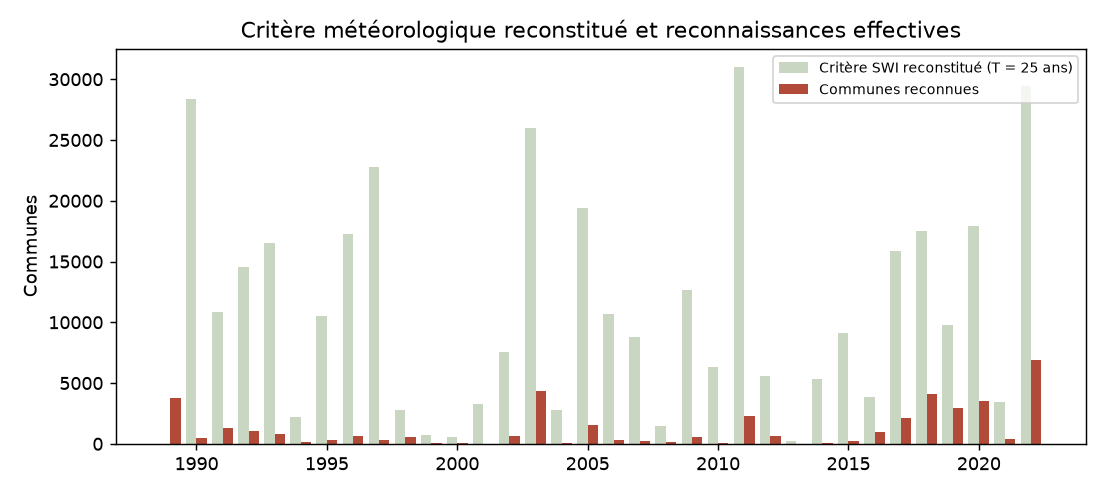
\includegraphics[width=.92\linewidth]{swi_critere.png}\caption{Communes satisfaisant le critère ($T=25$ ans) et communes effectivement reconnues.}\end{figure}

\section{Prévision du SWI uniforme d'été}
Cible : SWI moyen juin--août de la maille. Prédicteurs connus fin mai : SWI de mai et de mars--mai, hiver et été précédents, climatologie de la maille (années antérieures), tendance. Validation par origine glissante, test 1985--2026 ; la persistance et la climatologie sont les références.
\begin{table}[H]\centering\scriptsize\tabForecastAll\caption{Toutes années (RMSE et corrélation par maille ; \og nat. \fg{} : moyenne nationale annuelle).}\end{table}
\begin{table}[H]\centering\scriptsize\tabForecastDry\caption{Années sèches (quartile le plus sec).}\end{table}
Le modèle linéaire fait mieux que les modèles non linéaires : il extrapole la tendance climatique, que les arbres plafonnent.
\begin{figure}[H]\centering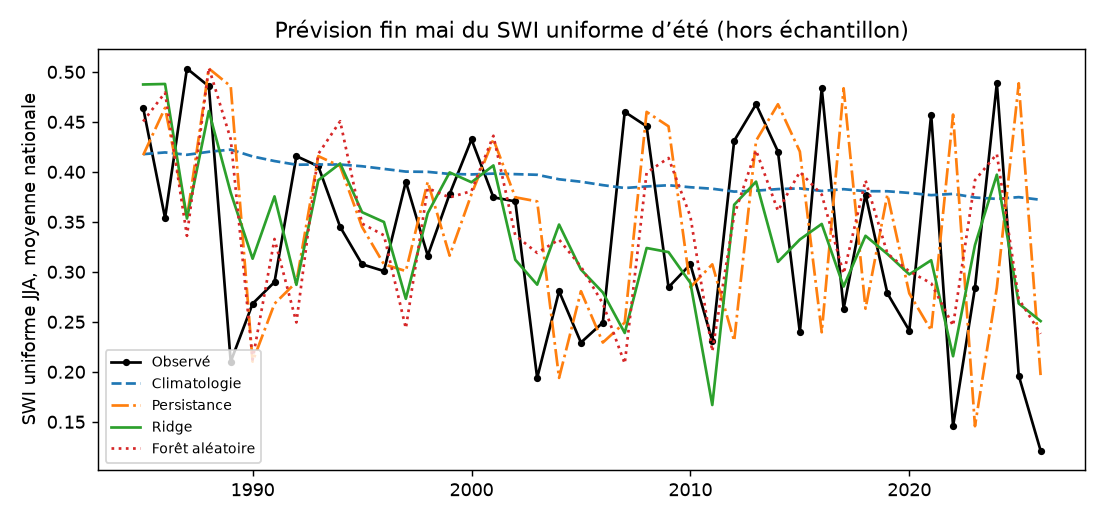
\includegraphics[width=.9\linewidth]{swi_prevision.png}\caption{Moyenne nationale du SWI d'été, observée et prévue.}\end{figure}

\section{Géostatistique}
Autocorrélation spatiale : $I$ de Moran $=$ \geoMoran. Variogramme ajusté par moindres carrés pondérés ; meilleur modèle : \geoBest. Krigeage ordinaire en voisinage glissant, validé en retirant des blocs spatiaux entiers (aucun voisin immédiat).
\begin{table}[H]\centering\small\tabVariogram\caption{Ajustements du variogramme (SWI uniforme d'été).}\end{table}
\begin{table}[H]\centering\small\tabKriging\caption{Validation du krigeage par blocs retirés. L'écart-type de l'erreur standardisée inférieur à 1 indique des intervalles légèrement prudents.}\end{table}
\begin{figure}[H]\centering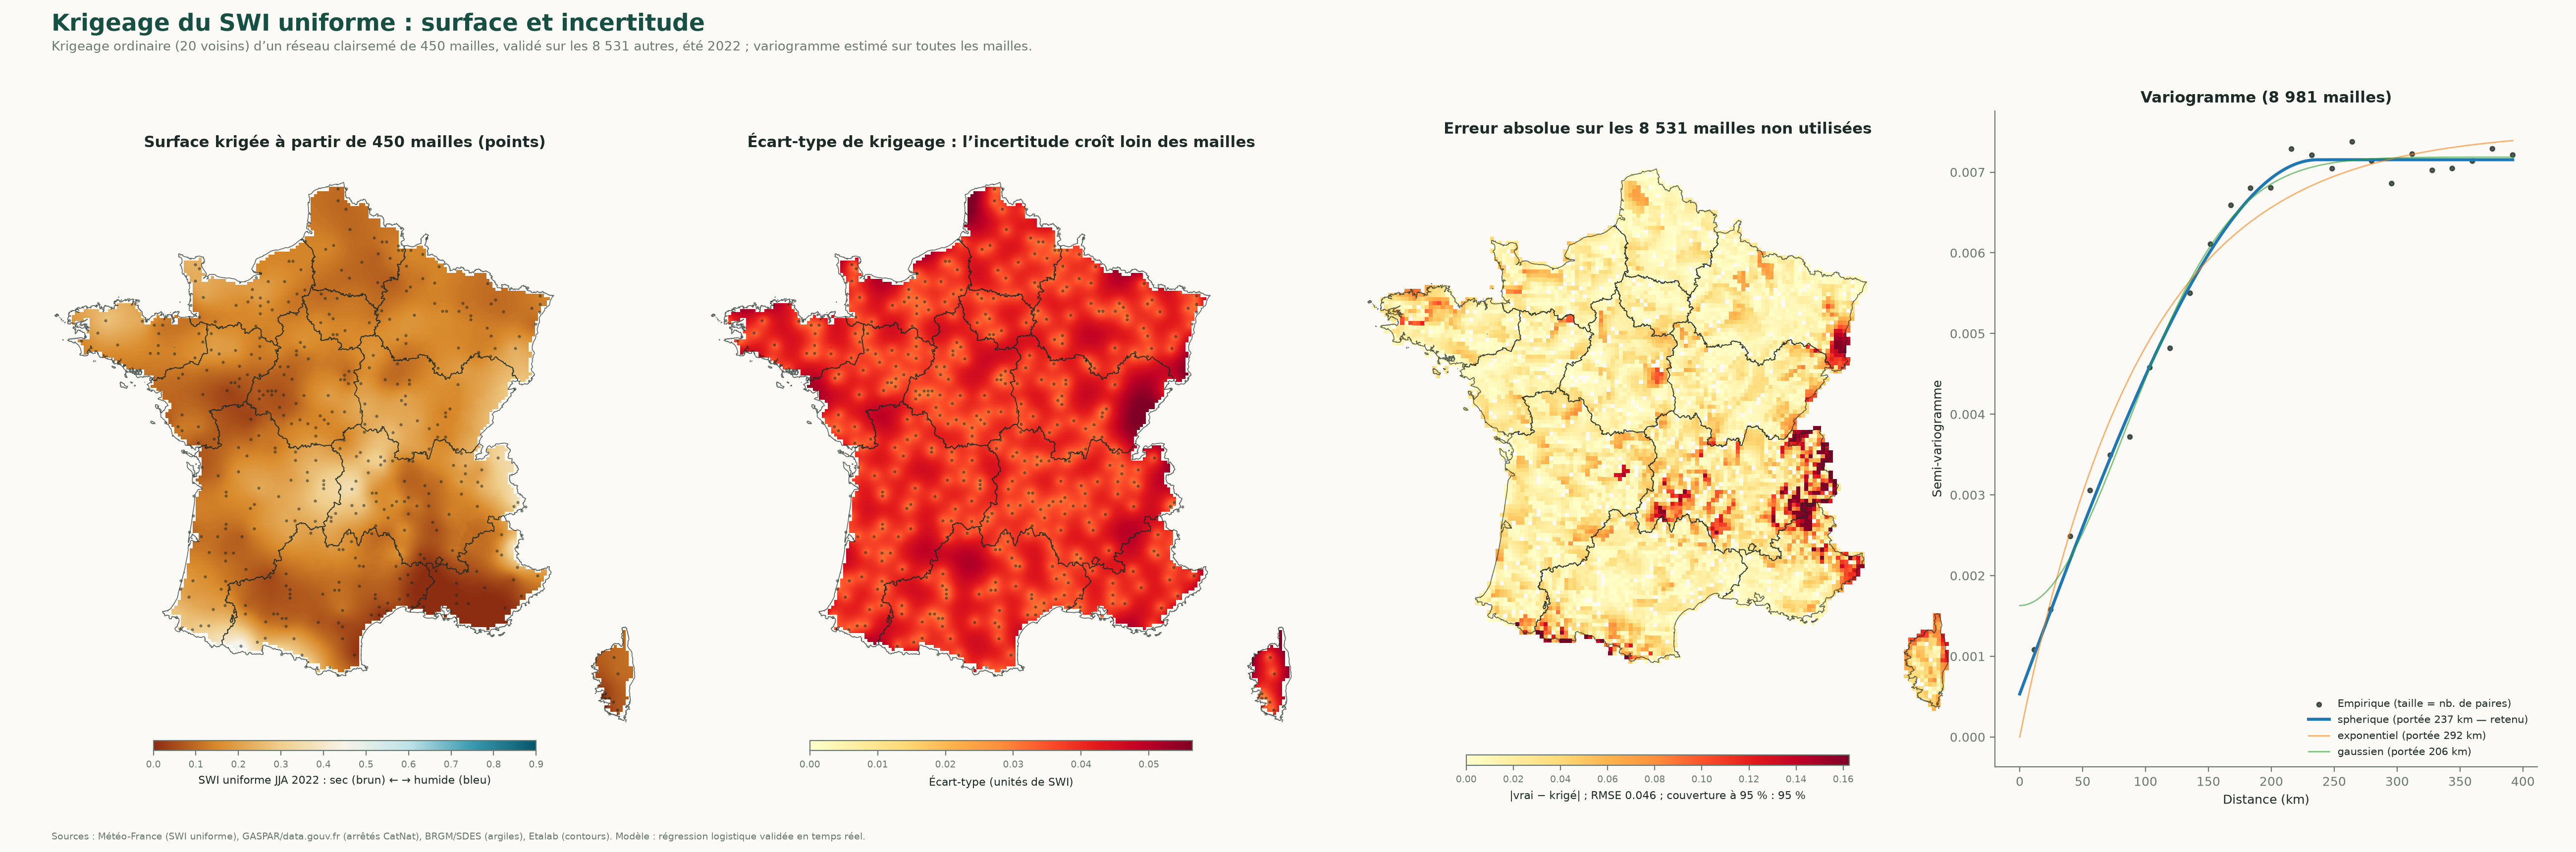
\includegraphics[width=\linewidth]{pro_krigeage_swi.png}\caption{Krigeage du SWI uniforme d'été 2022 à partir de 450 mailles : surface, écart-type, erreur réelle sur les 8\,531 mailles non utilisées et variogramme. La couverture de l'intervalle à 95\,\% est de 95\,\%.}\end{figure}

\section{Estimer le SWI uniforme là où il n'existe pas}
Le SWI uniforme n'existe qu'aux 8\,981 mailles de 8\,km. Une commune se situe entre mailles : plutôt que de lui attribuer la maille la plus proche, on estime son SWI \emph{au centre de la commune} par krigeage ordinaire en voisinage glissant (24 mailles). Les poids de krigeage ne dépendent que de la géométrie et du variogramme : ils sont calculés une fois par commune puis appliqués à toute la série mensuelle (1959--2026) ; le variogramme est celui de champs d'été standardisés, ajusté sur les distances inférieures à 100\,km (modèle exponentiel, retenu par validation). Résumé : \interpSummary.
\begin{table}[H]\centering\small\tabInterp\caption{Validation par retrait de 10\,\% des mailles au hasard (SWI uniforme d'été, unités de SWI). Les intervalles du krigeage sont bien calibrés.}\end{table}
\begin{table}[H]\centering\small\tabInterpModel\caption{Effet sur le modèle de fréquence : indicateurs de la maille la plus proche contre indicateurs du SWI krigé au centre des communes.}\end{table}
\begin{figure}[H]\centering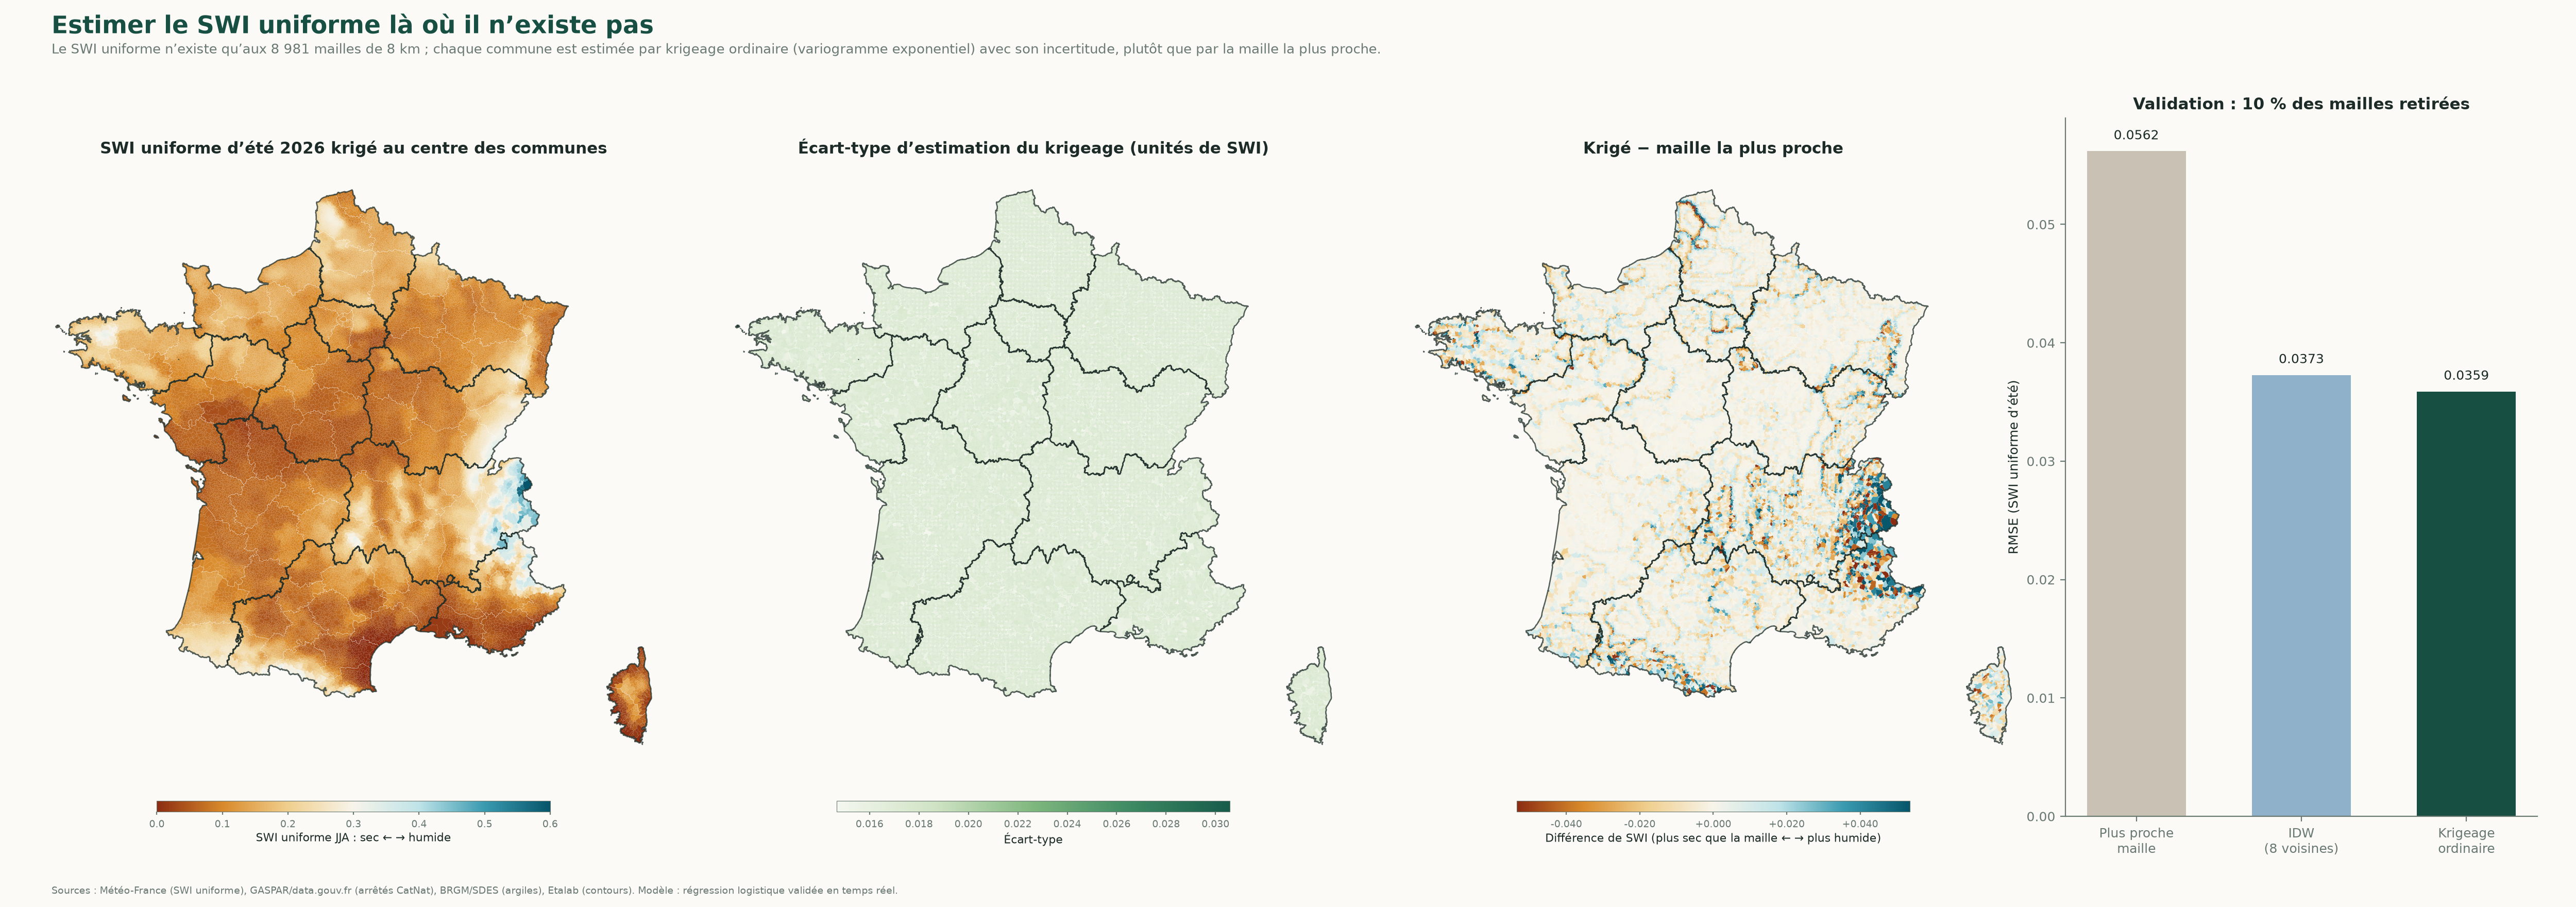
\includegraphics[width=\linewidth]{pro_interpolation_communes.png}\caption{SWI uniforme d'été 2026 krigé au centre des communes, incertitude d'estimation, écart avec la maille la plus proche et comparaison des méthodes.}\end{figure}
Le krigeage réduit l'erreur d'environ 36\,\% par rapport à la maille la plus proche et fait légèrement mieux que la pondération inverse, avec un intervalle d'incertitude calibré, que l'IDW ne fournit pas. Les corrections sont les plus fortes en relief (Alpes). Au niveau du modèle de fréquence le gain est modeste : les centres de communes sont en moyenne à 3\,km d'une maille.

\section{Climat : tendances et sensibilité}
Ces éléments ne sont \emph{pas} des projections climatiques (pas de scénarios DRIAS/CMIP) : ce sont les tendances observées dans la réanalyse SIM et des tests de sensibilité du modèle. Tendance du SWI d'été moyen national (Theil--Sen) : \climateTrend.
\begin{table}[H]\centering\small\tabClimateDecades\caption{Part des mailles dont l'été passe sous le décile de leur référence 1959--1988 (10\,\% par construction sur la référence).}\end{table}
\begin{figure}[H]\centering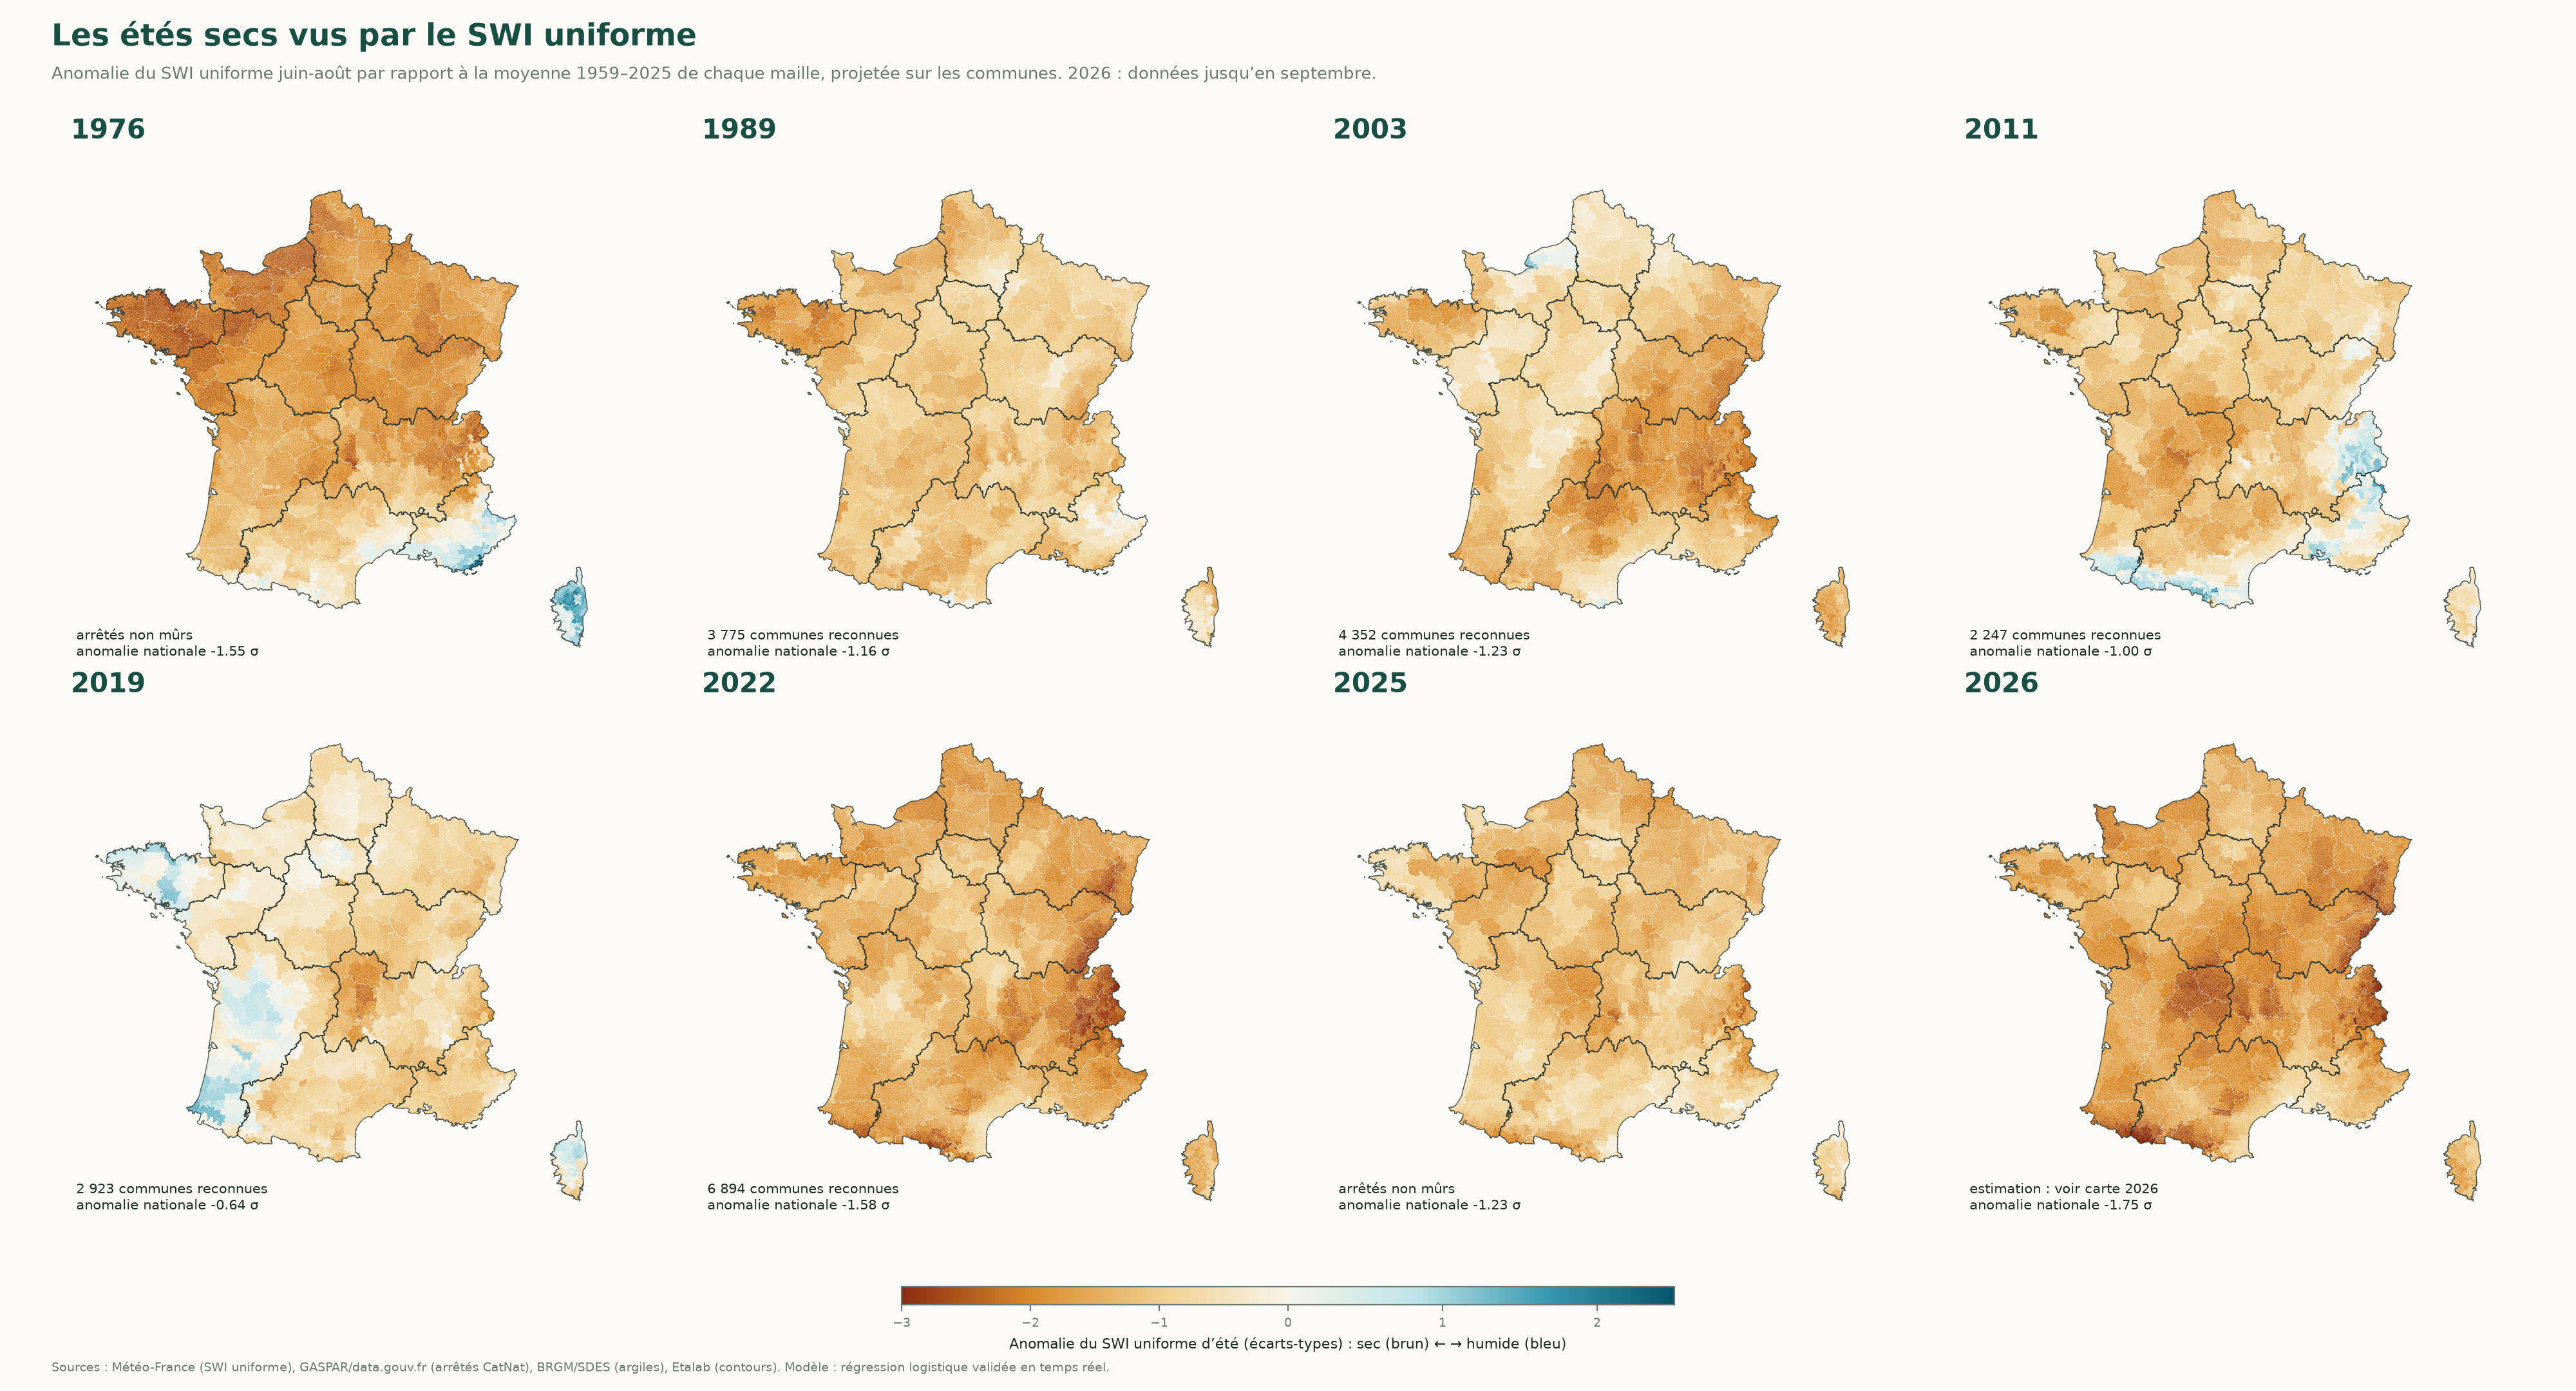
\includegraphics[width=\linewidth]{pro_swi_etes_secs.png}\caption{Anomalie du SWI uniforme d'été de huit années marquantes, projetée sur les communes.}\end{figure}
\begin{figure}[H]\centering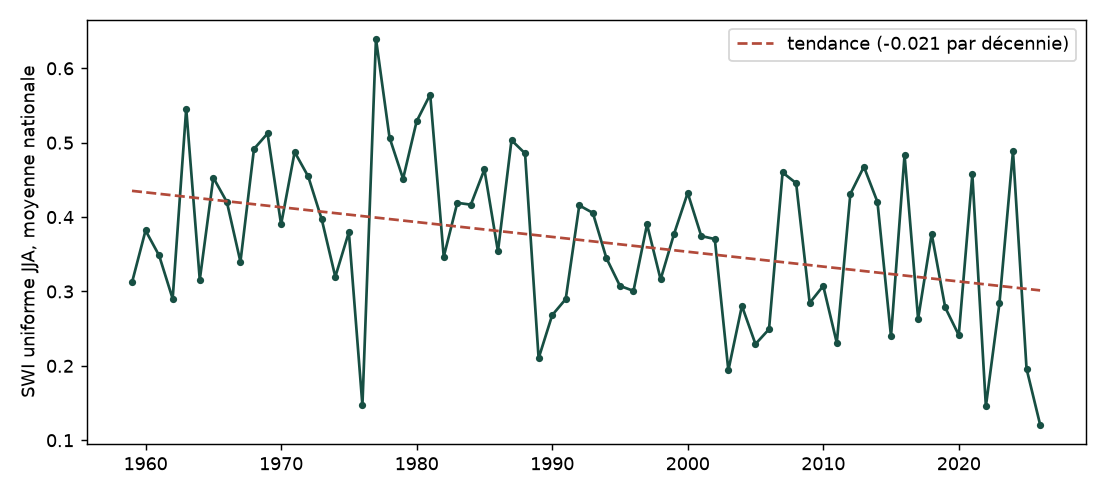
\includegraphics[width=.85\linewidth]{climate_tendance.png}\caption{SWI uniforme d'été, moyenne nationale, et tendance.}\end{figure}
\begin{table}[H]\centering\small\tabSensitivity\caption{Communes reconnues attendues si le SWI d'une année de base est déplacé de façon uniforme (modèle appris sur les années $\le t-2$).}\end{table}

\section{Modèle de fréquence}
Régressions logistiques de complexité croissante et gradient boosting, comparées à une fréquence constante et à une fréquence communale crédibilisée ($k=3$). Indicateurs sans information future (climatologie expansive), historique limité aux arrêtés \emph{publiés} avant l'année prédite, validation en temps réel 1995--2022.
\begin{table}[H]\centering\small\tabModels\caption{Scores hors échantillon 1995--2022 (log-loss, gain relatif à la constante, Brier, AUC, communes attendues).}\end{table}
\begin{table}[H]\centering\small\tabModelsRecent\caption{Sous-période 2010--2022.}\end{table}
\begin{table}[H]\centering\scriptsize\tabByYear\caption{Observé contre attendu par année (GLM complet) : la classification est bonne (AUC), le niveau annuel non.}\end{table}
\begin{table}[H]\centering\small\tabCoef\caption{Coefficients du GLM complet, variables standardisées. Les indicateurs météo sont corrélés : lecture conjointe.}\end{table}
\begin{figure}[H]\centering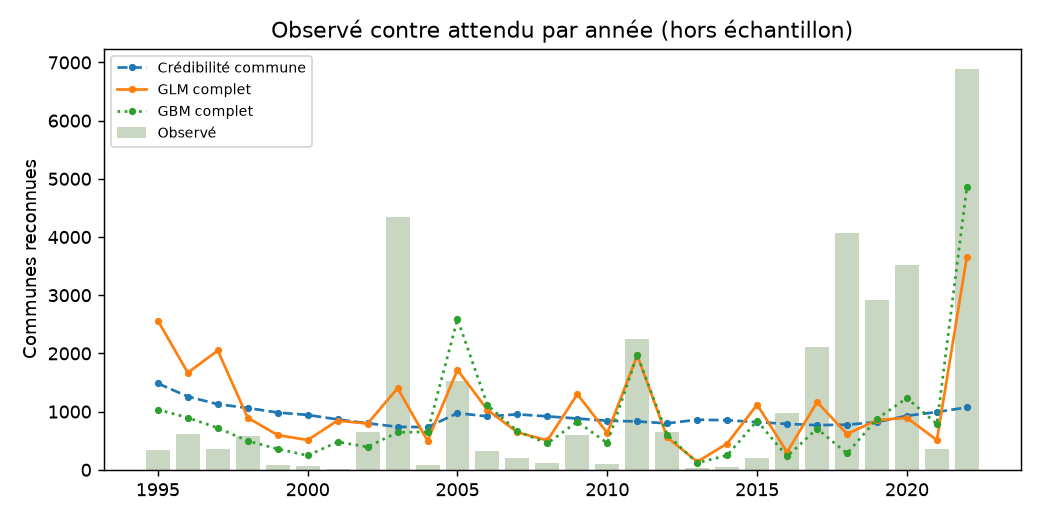
\includegraphics[width=.9\linewidth]{observe_attendu.png}\caption{Communes reconnues par année : observé et attendu hors échantillon.}\end{figure}

\begin{figure}[H]\centering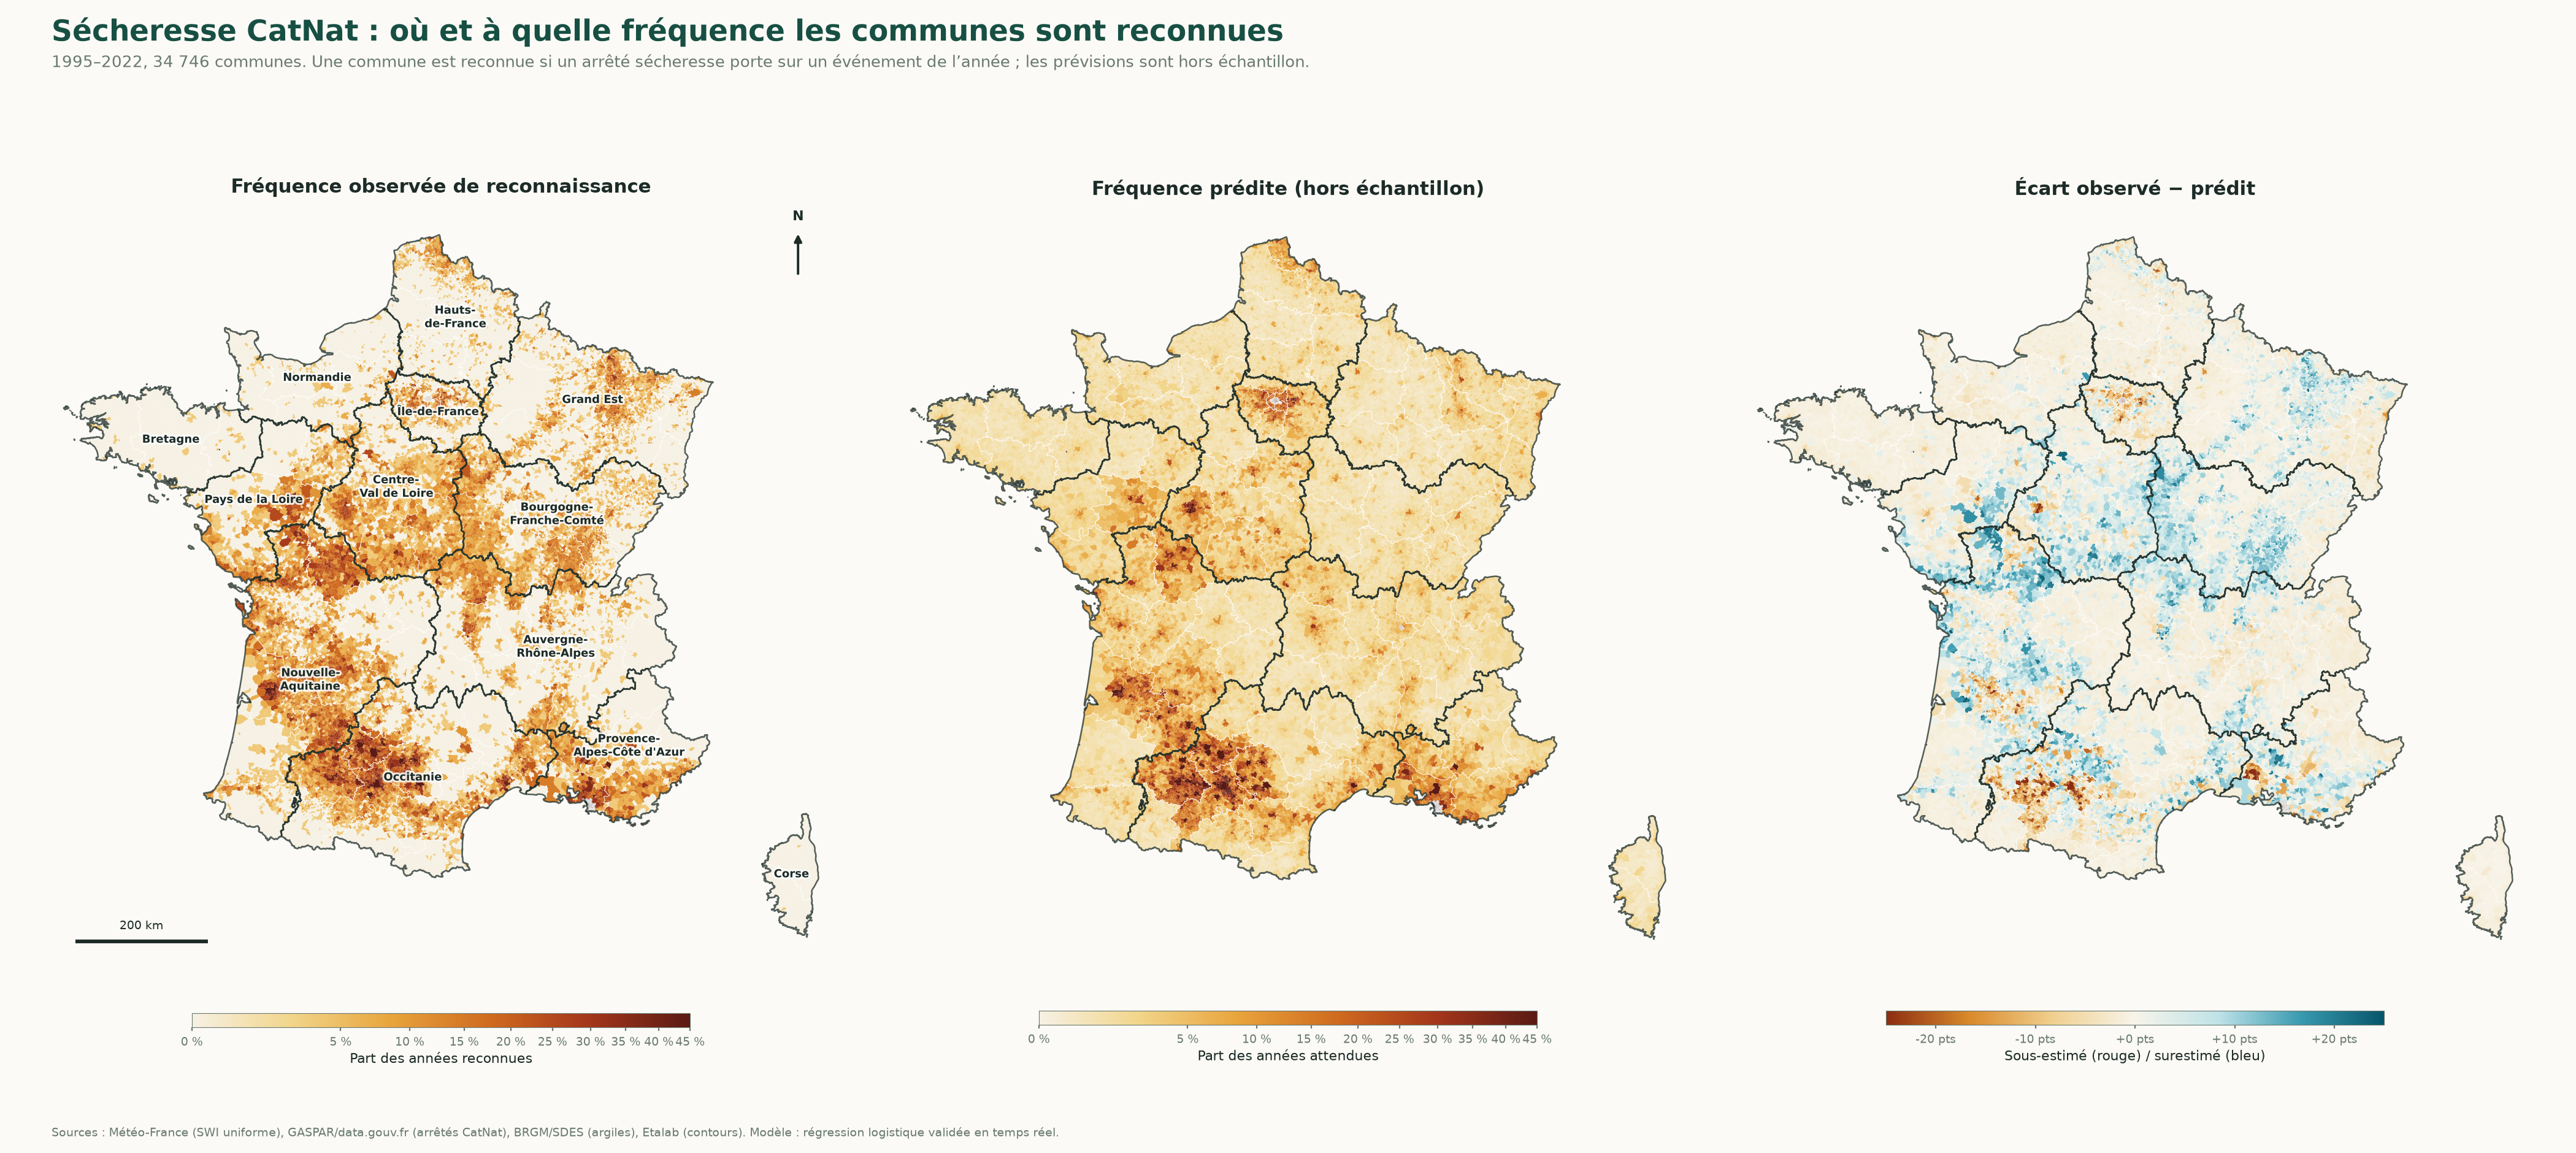
\includegraphics[width=\linewidth]{pro_france_triptyque.png}\caption{Fréquence de reconnaissance par commune : observée, prédite hors échantillon, écart.}\end{figure}
\begin{figure}[H]\centering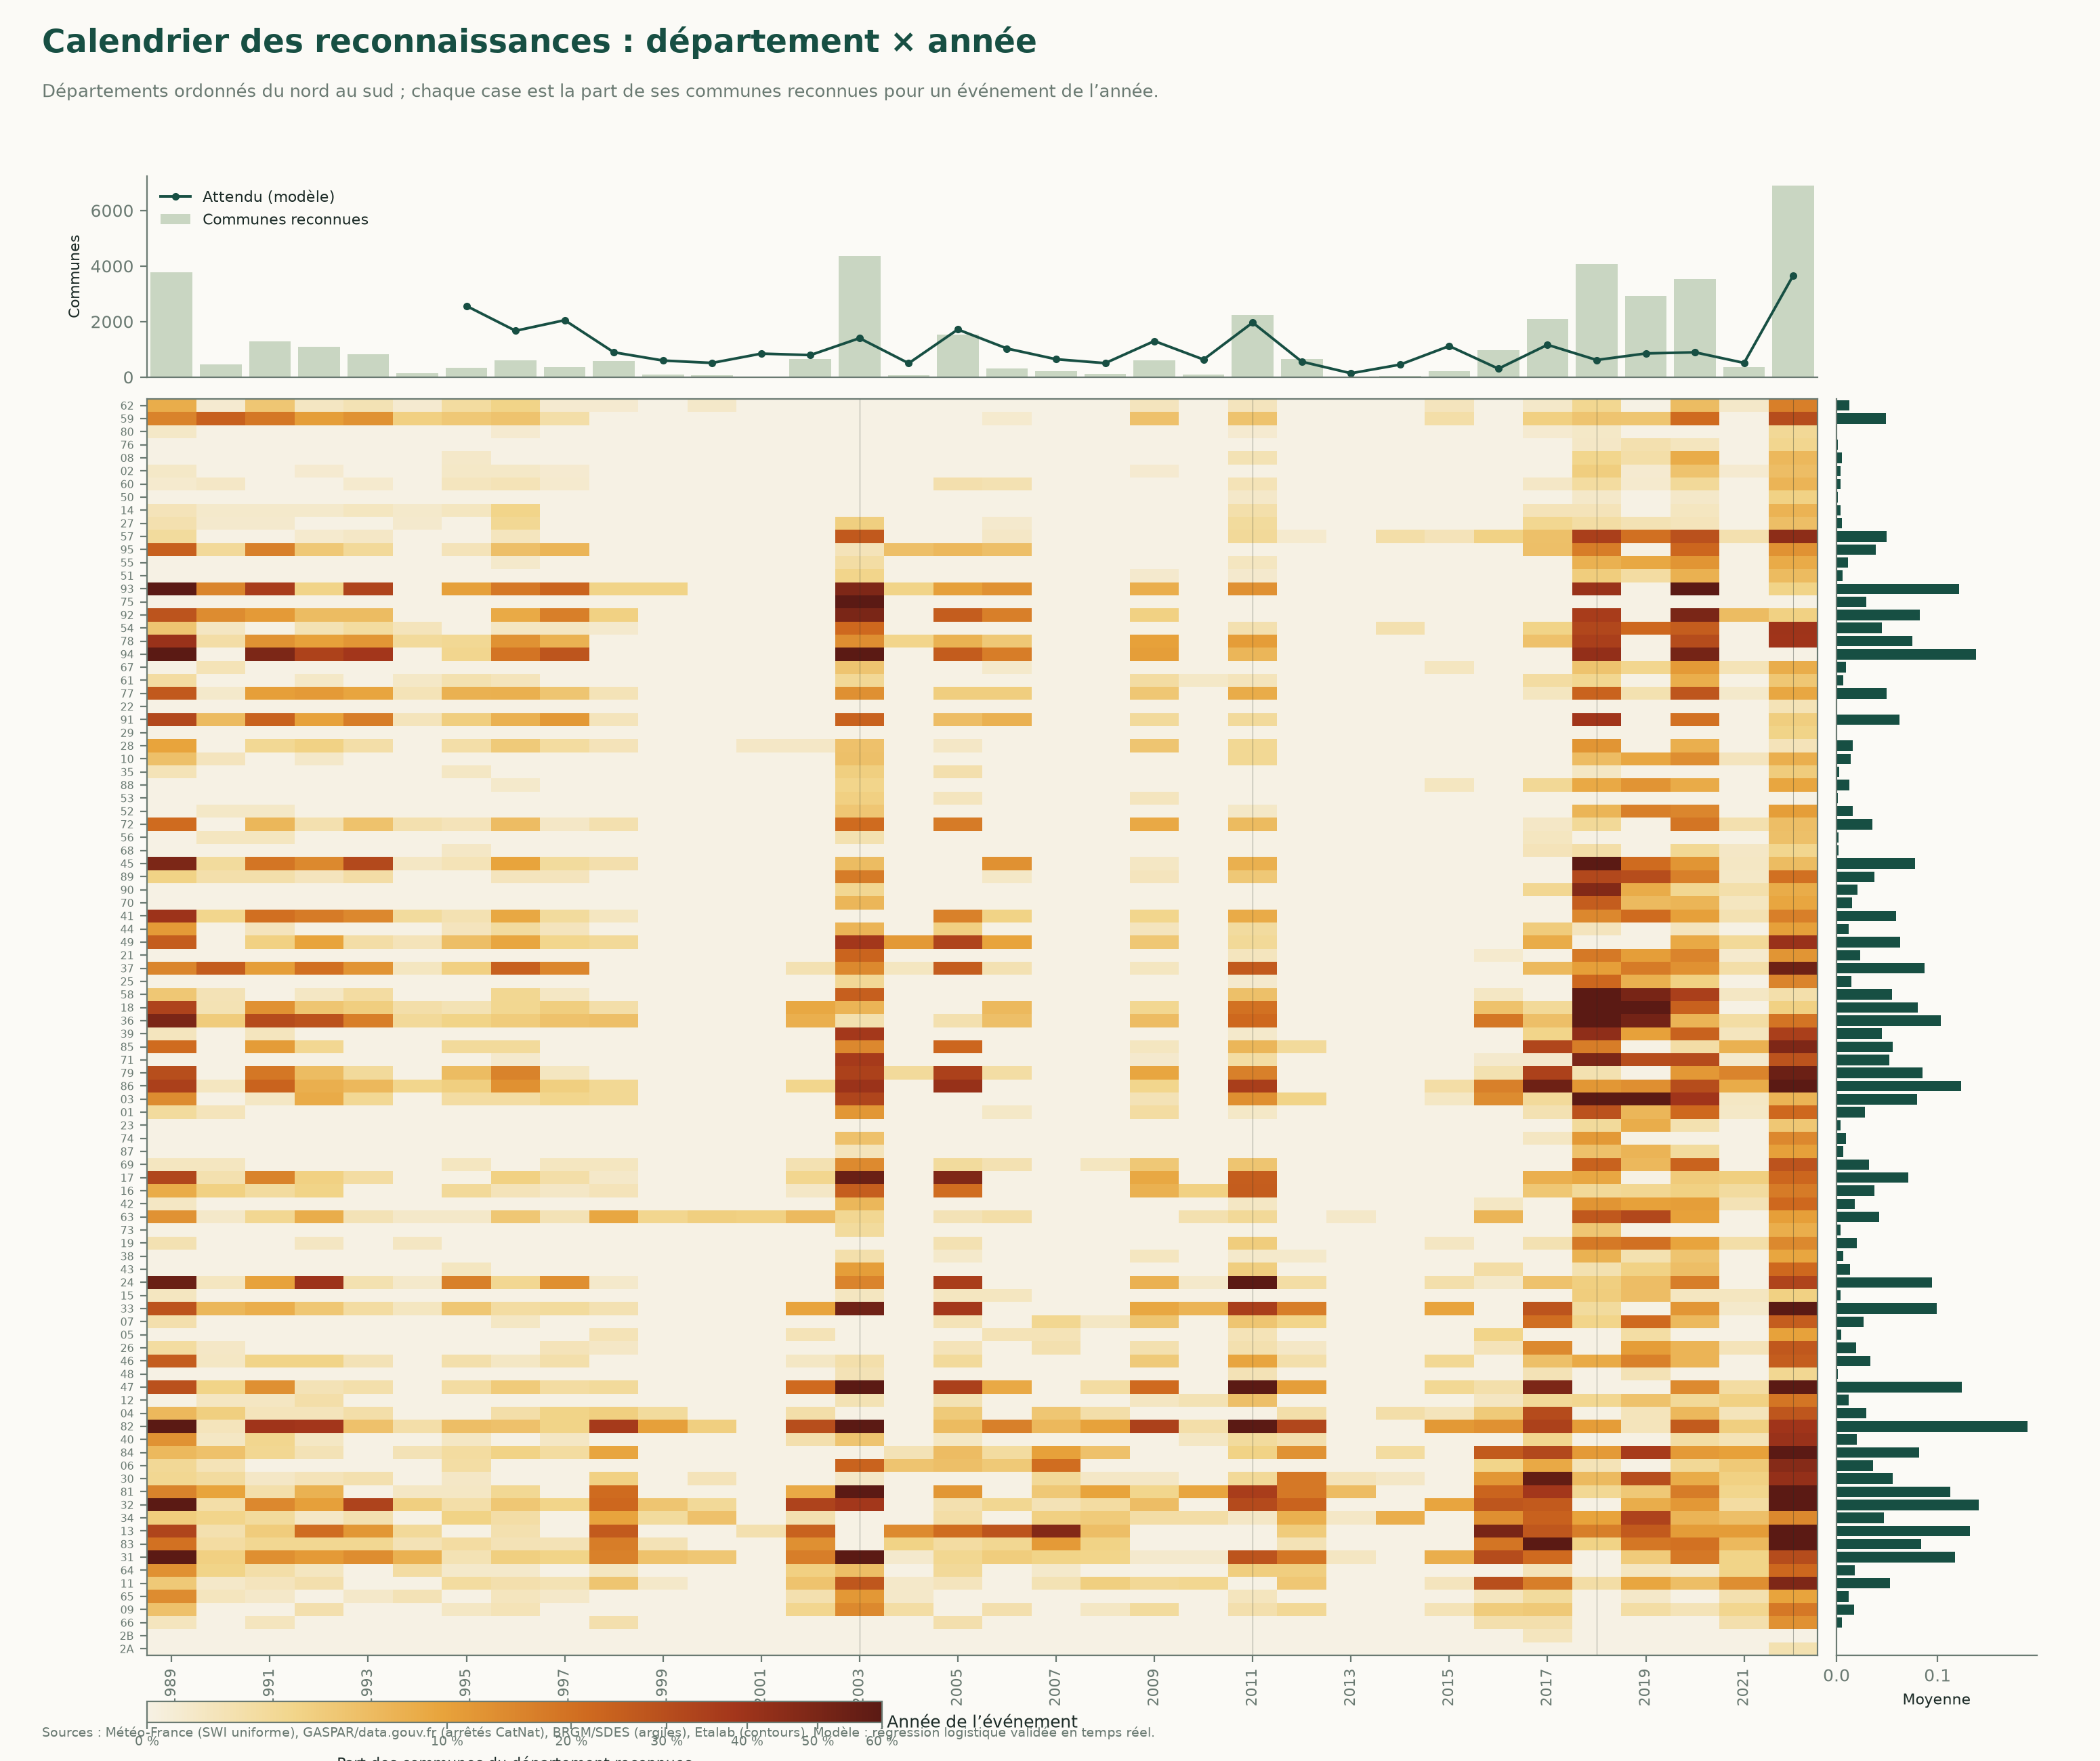
\includegraphics[width=.95\linewidth]{pro_calendrier_departements.png}\caption{Calendrier département $\times$ année des communes reconnues.}\end{figure}

\subsection*{Aléa argile communal}
L'exposition par EPCI est grossière. La carte d'exposition BRGM 2025 (121\,399 polygones, aléas faible, moyen, fort) est superposée aux contours des communes pour obtenir, pour chaque commune, la \emph{part de sa surface} dans chaque classe. Son apport est lisible dans les tableaux ci-dessus (modèles \og + aléa argile communal \fg) : c'est l'amélioration la plus nette. Une vérification sur les 119 communes du 13 l'avait annoncée.
\begin{figure}[H]\centering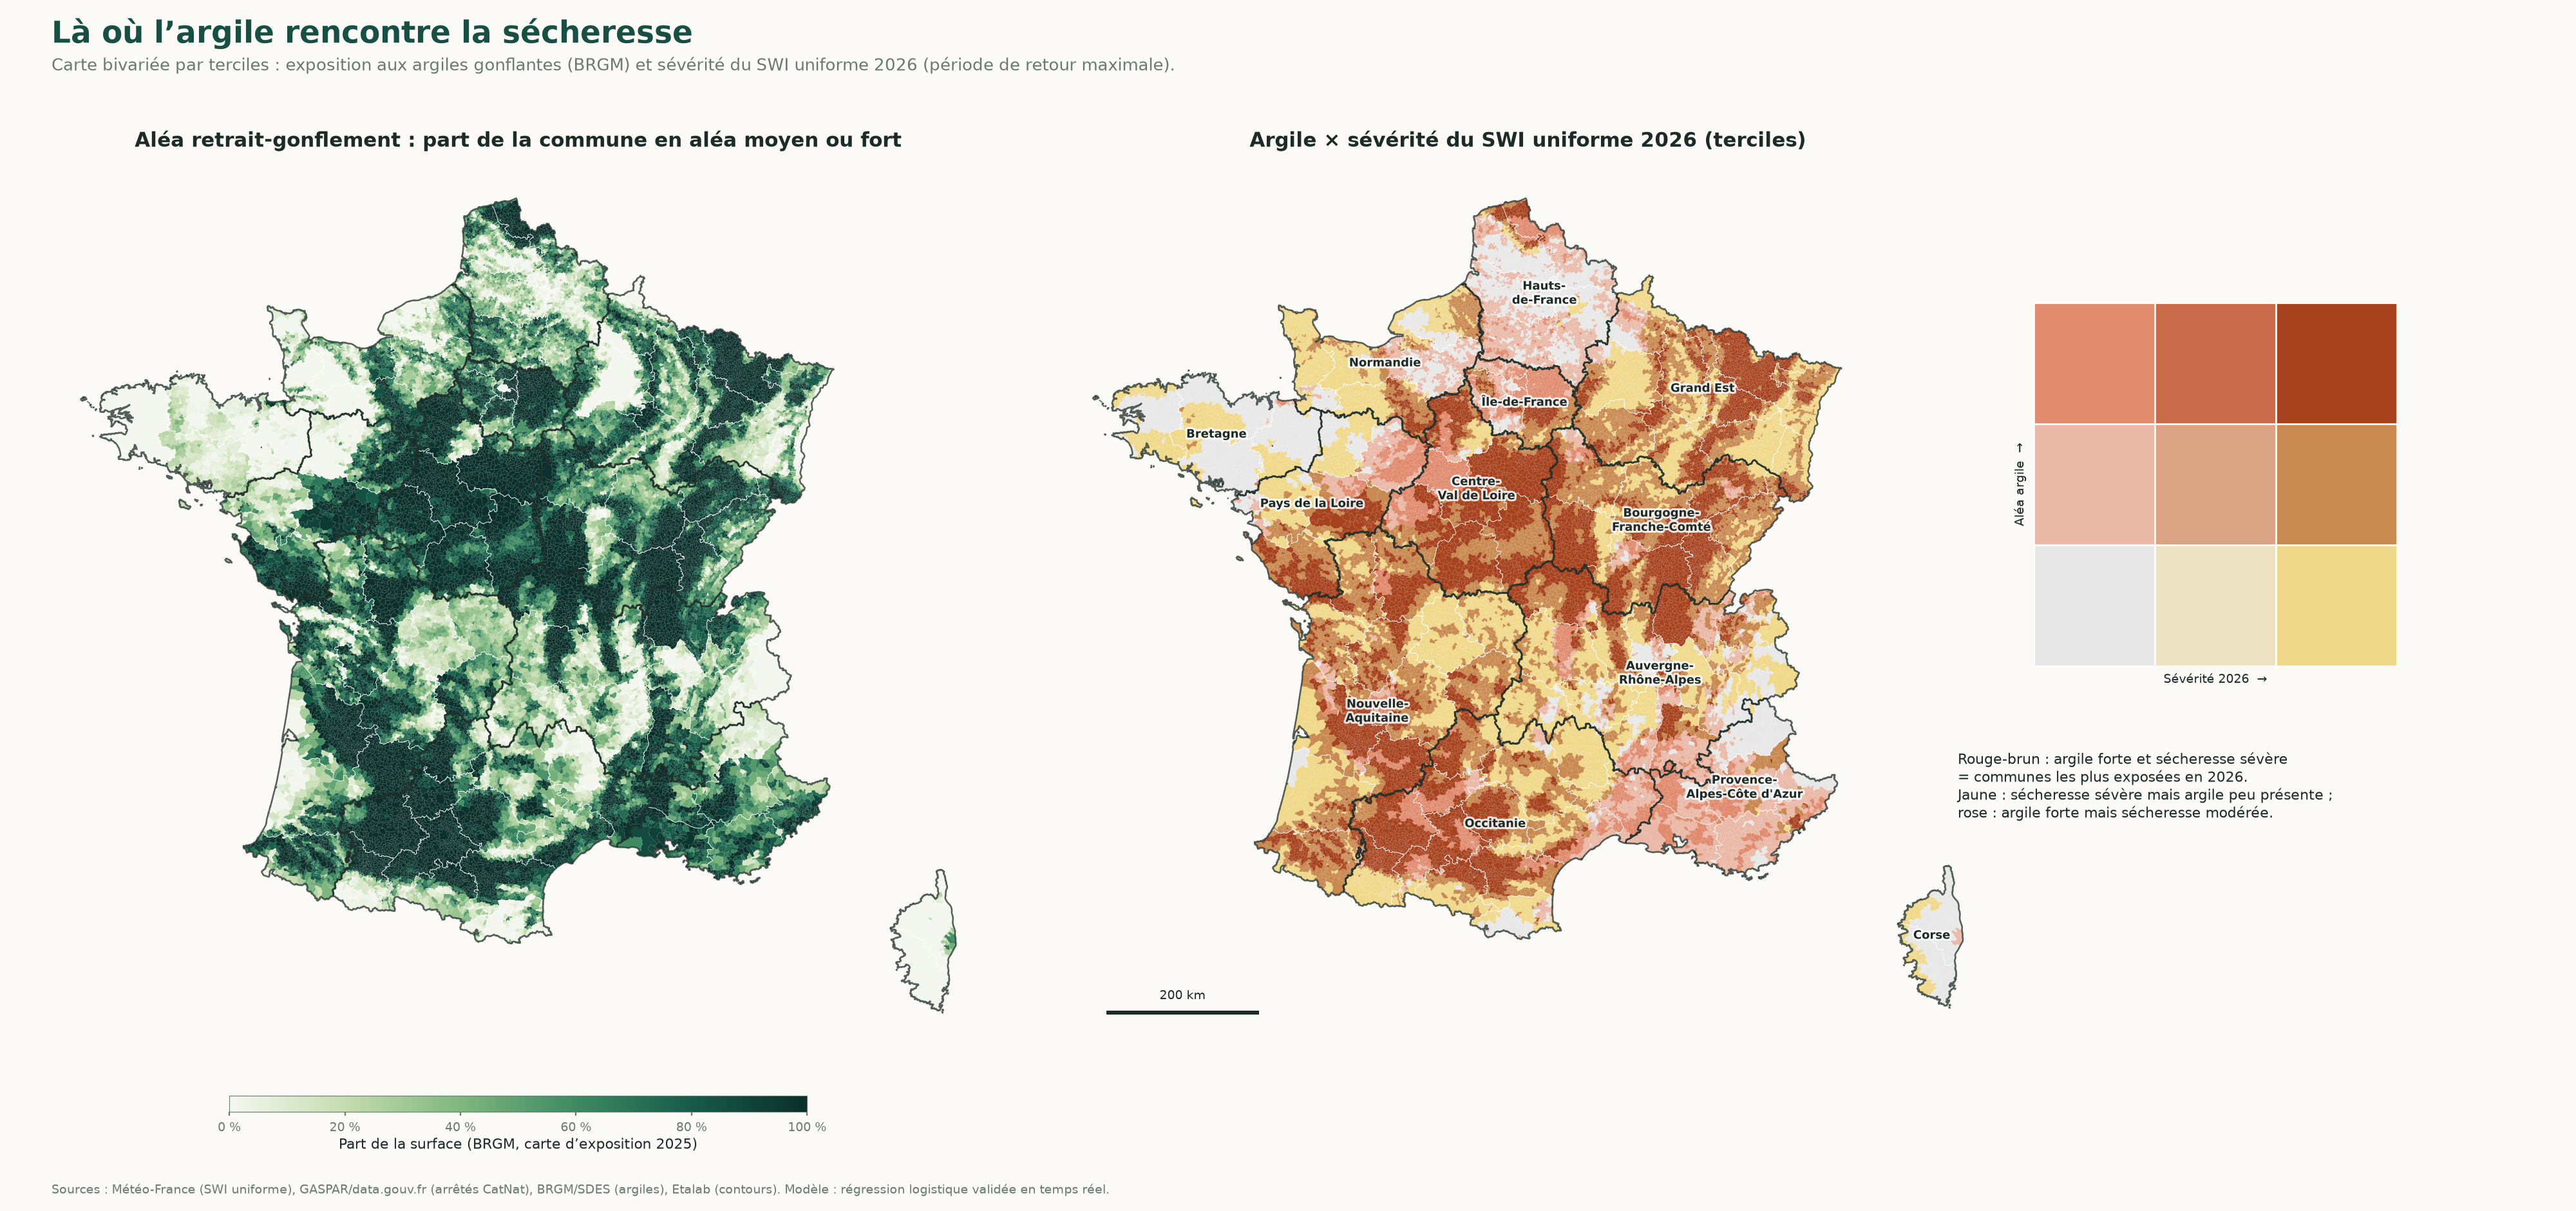
\includegraphics[width=\linewidth]{pro_bivarie_argile_secheresse.png}\caption{Carte bivariée par terciles : part communale en aléa argile moyen ou fort et sévérité du SWI uniforme 2026.}\end{figure}
\begin{table}[H]\centering\small\tabOldScore\caption{Ancien score composite du Drive et indicateurs, contre la fréquence réelle de reconnaissance 1989--2022 des communes du 13.}\end{table}

\section{Cartes}
\begin{figure}[H]\centering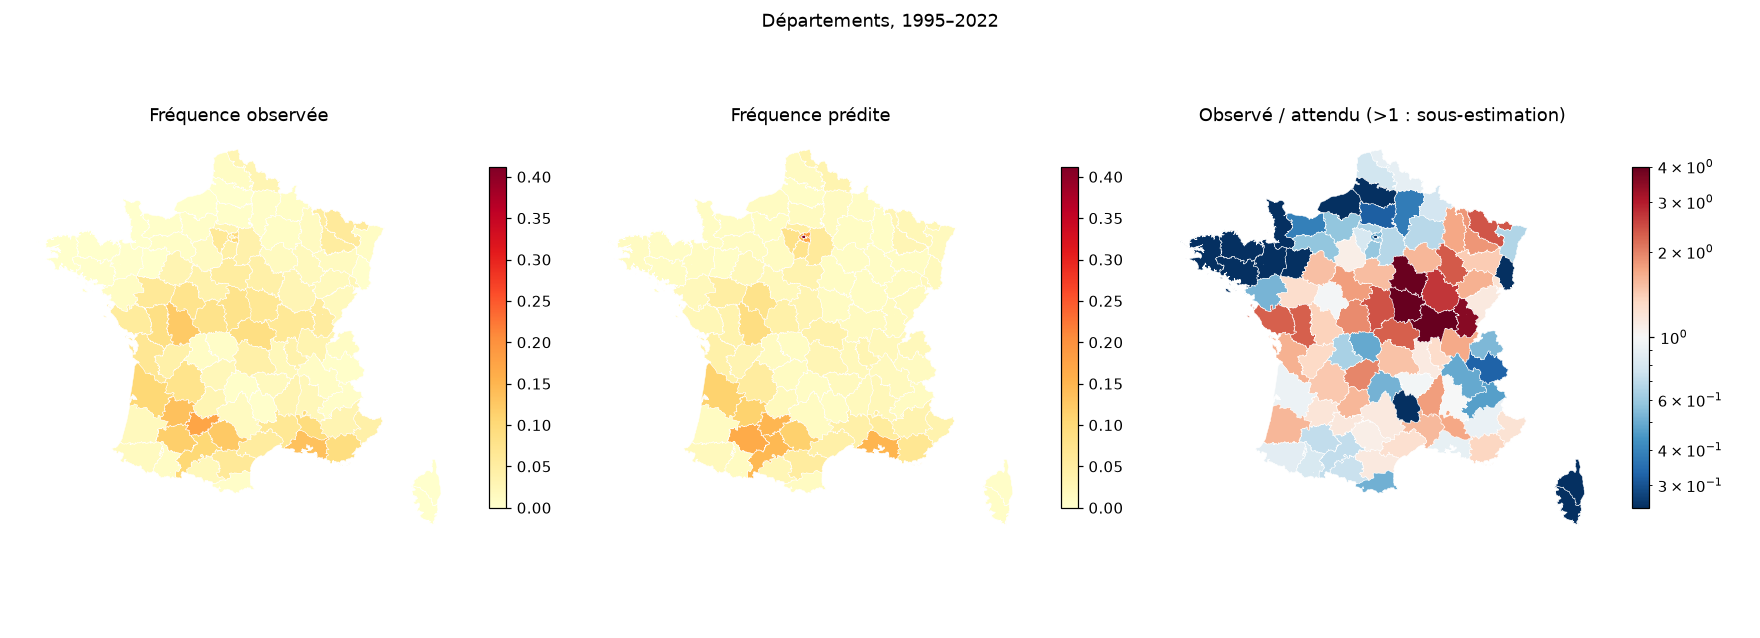
\includegraphics[width=\linewidth]{carte_departements.png}\caption{Fréquence observée, prédite et rapport observé/attendu par département.}\end{figure}
\begin{table}[H]\centering\small\tabDept\caption{Départements les plus sous-estimés.}\end{table}
\begin{figure}[H]\centering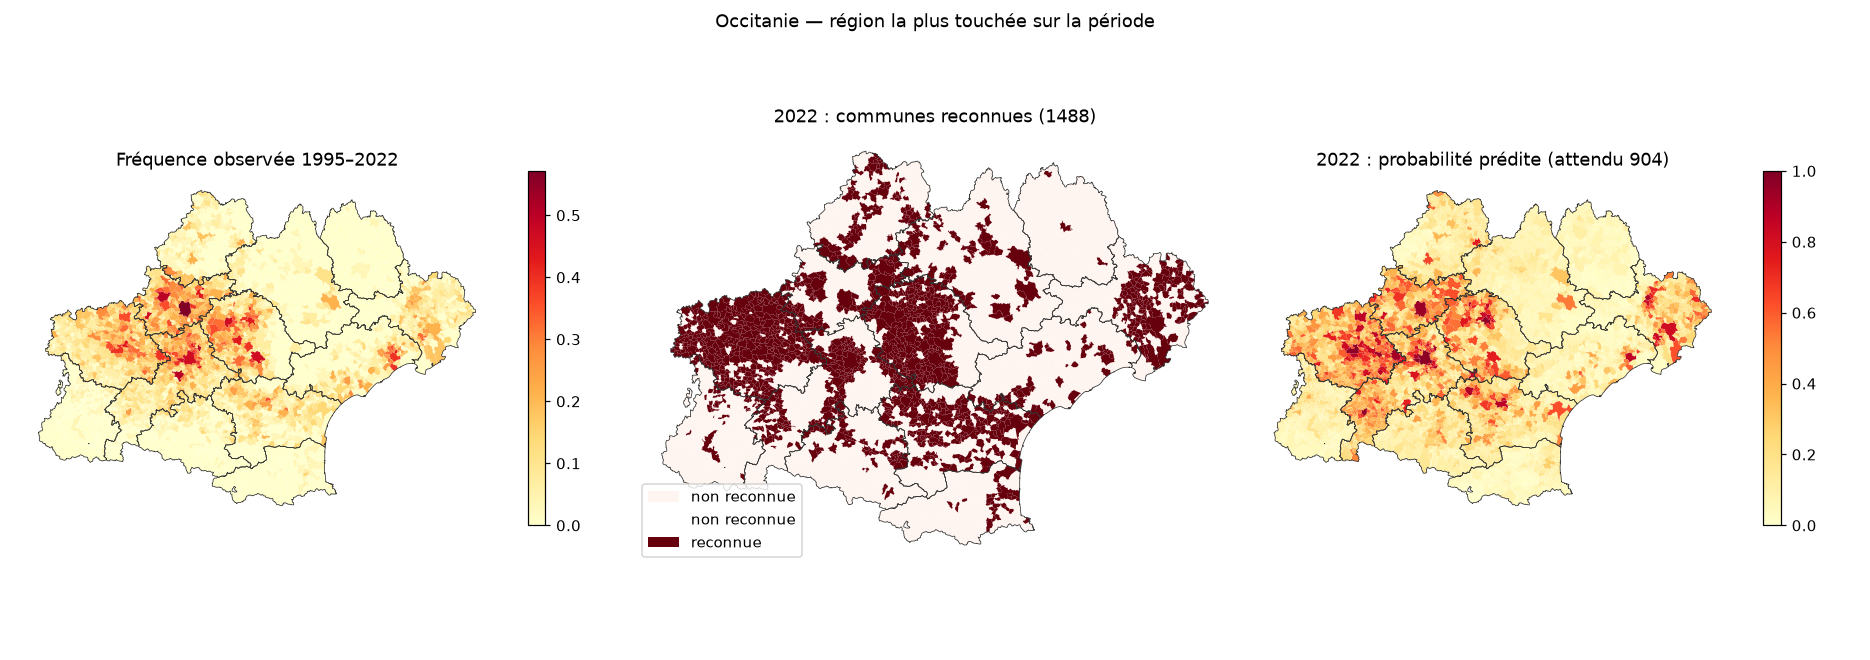
\includegraphics[width=\linewidth]{carte_region_76.png}\caption{Occitanie, région la plus touchée sur la période.}\end{figure}

\section{Résultat 2026 avec intervalles}
Données SWI uniforme jusqu'en septembre 2026 ; arrêtés non publiés. \nowcastSummary. Deux intervalles distincts : le premier mesure l'incertitude statistique (bootstrap par blocs d'années), le second l'erreur de niveau annuel observée sur le backtest.
\begin{table}[H]\centering\small\tabIntervals\caption{Estimation 2026 et intervalles. La couverture est mesurée en laissant chaque année de côté.}\end{table}
\begin{table}[H]\centering\small\tabSeverity\caption{2026 comparée aux années les plus sévères de la série.}\end{table}
\begin{table}[H]\centering\small\tabRegionsNow\caption{Régions les plus exposées en 2026 (estimation).}\end{table}
\begin{figure}[H]\centering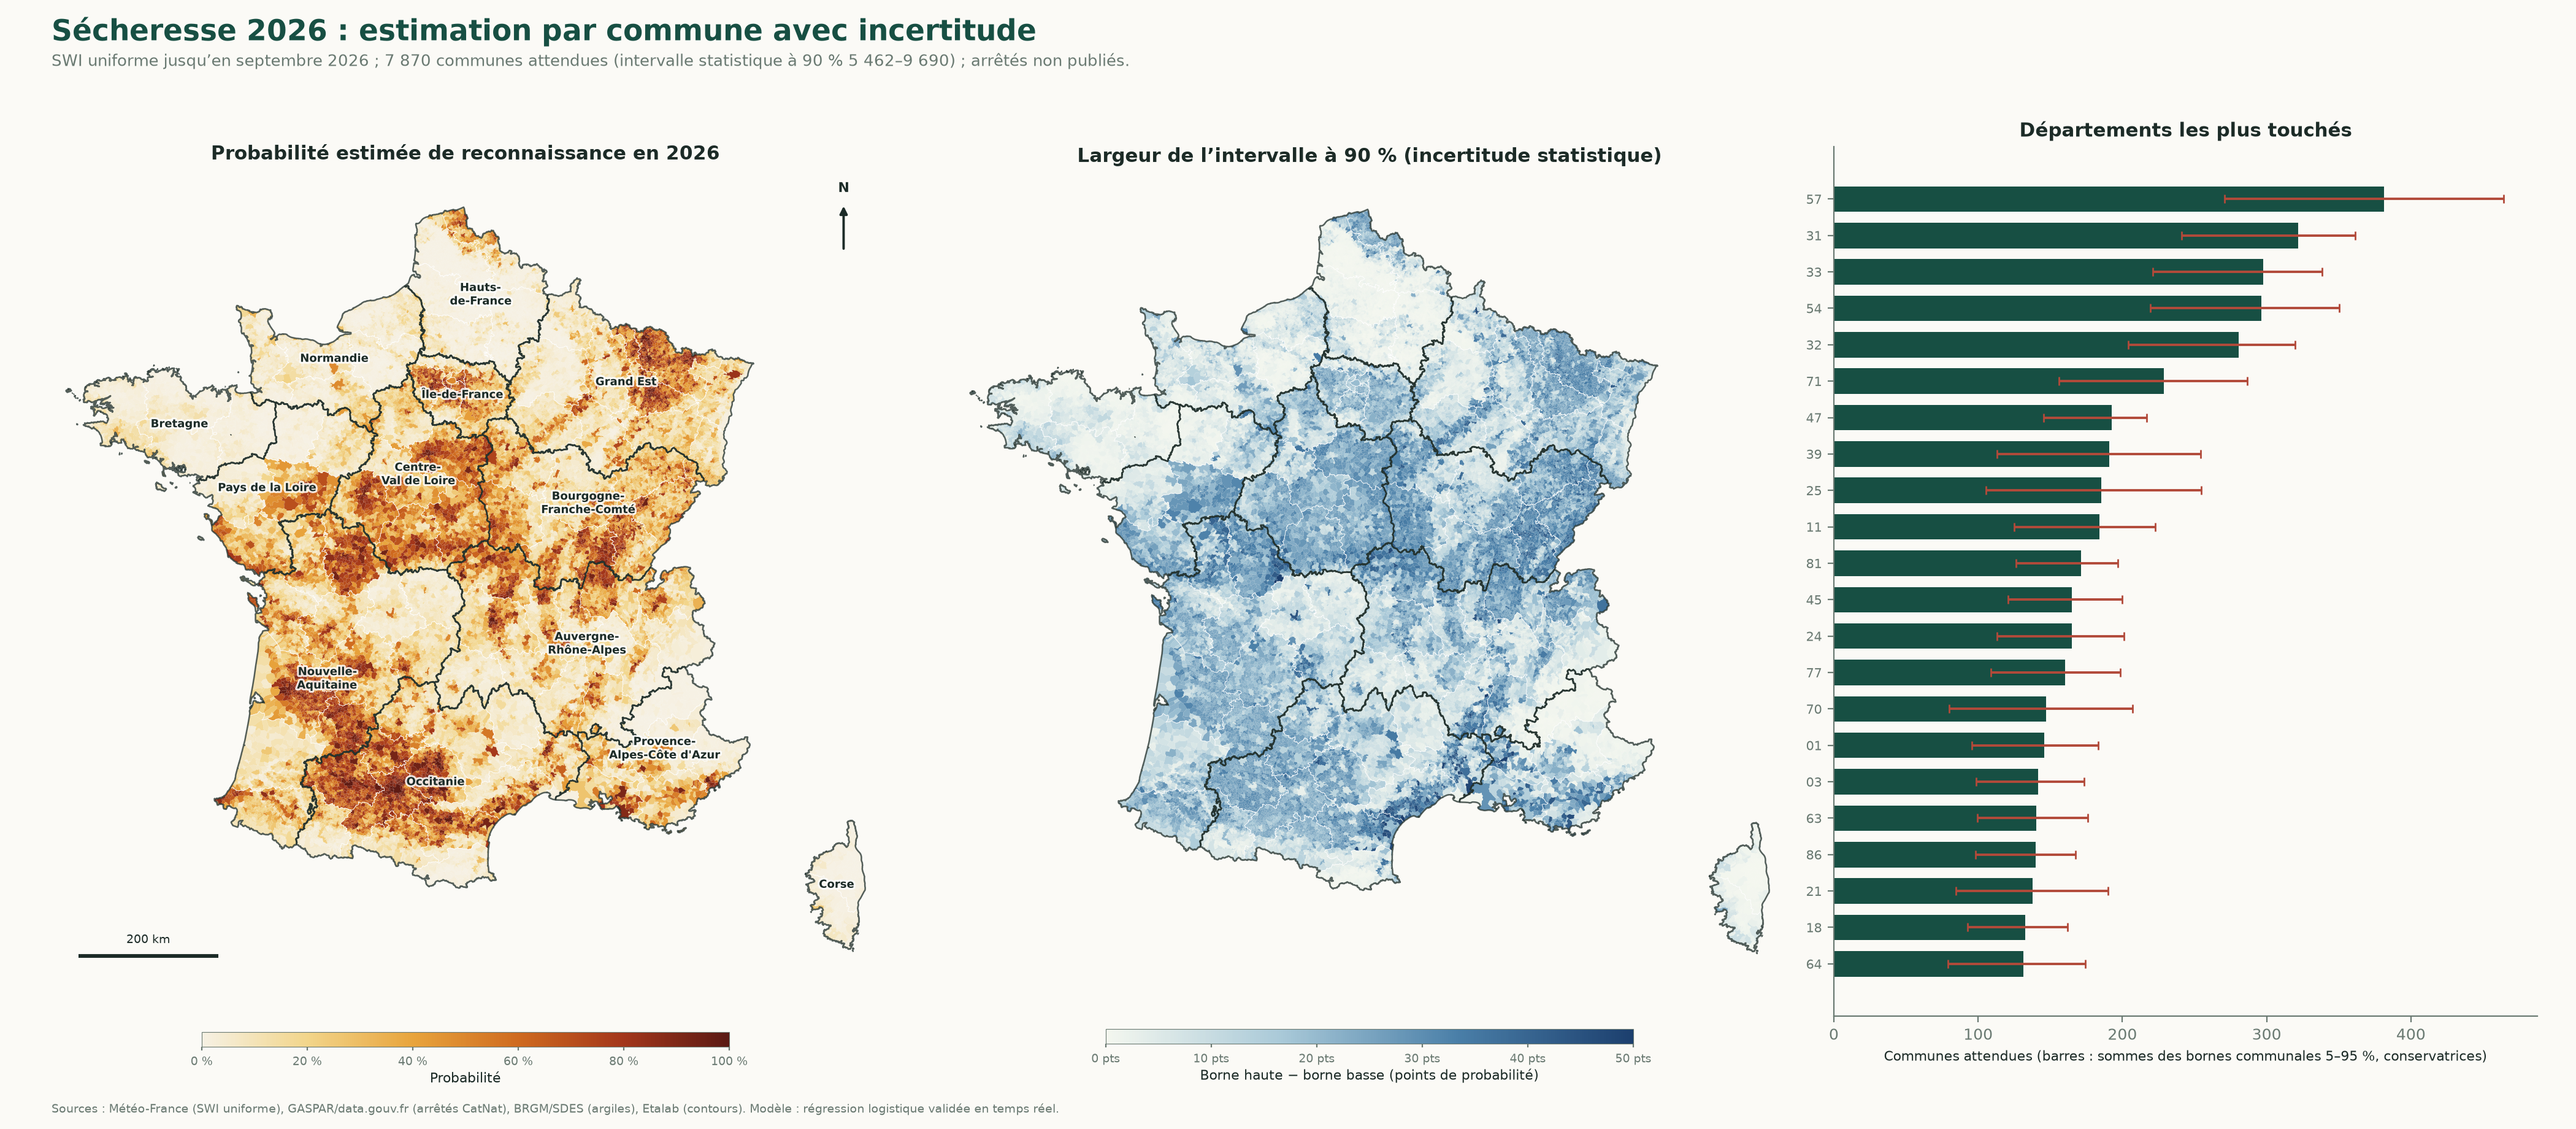
\includegraphics[width=\linewidth]{pro_nowcast_2026.png}\caption{Probabilité estimée de reconnaissance en 2026, largeur de l'intervalle à 90\,\% et départements les plus touchés.}\end{figure}
\begin{figure}[H]\centering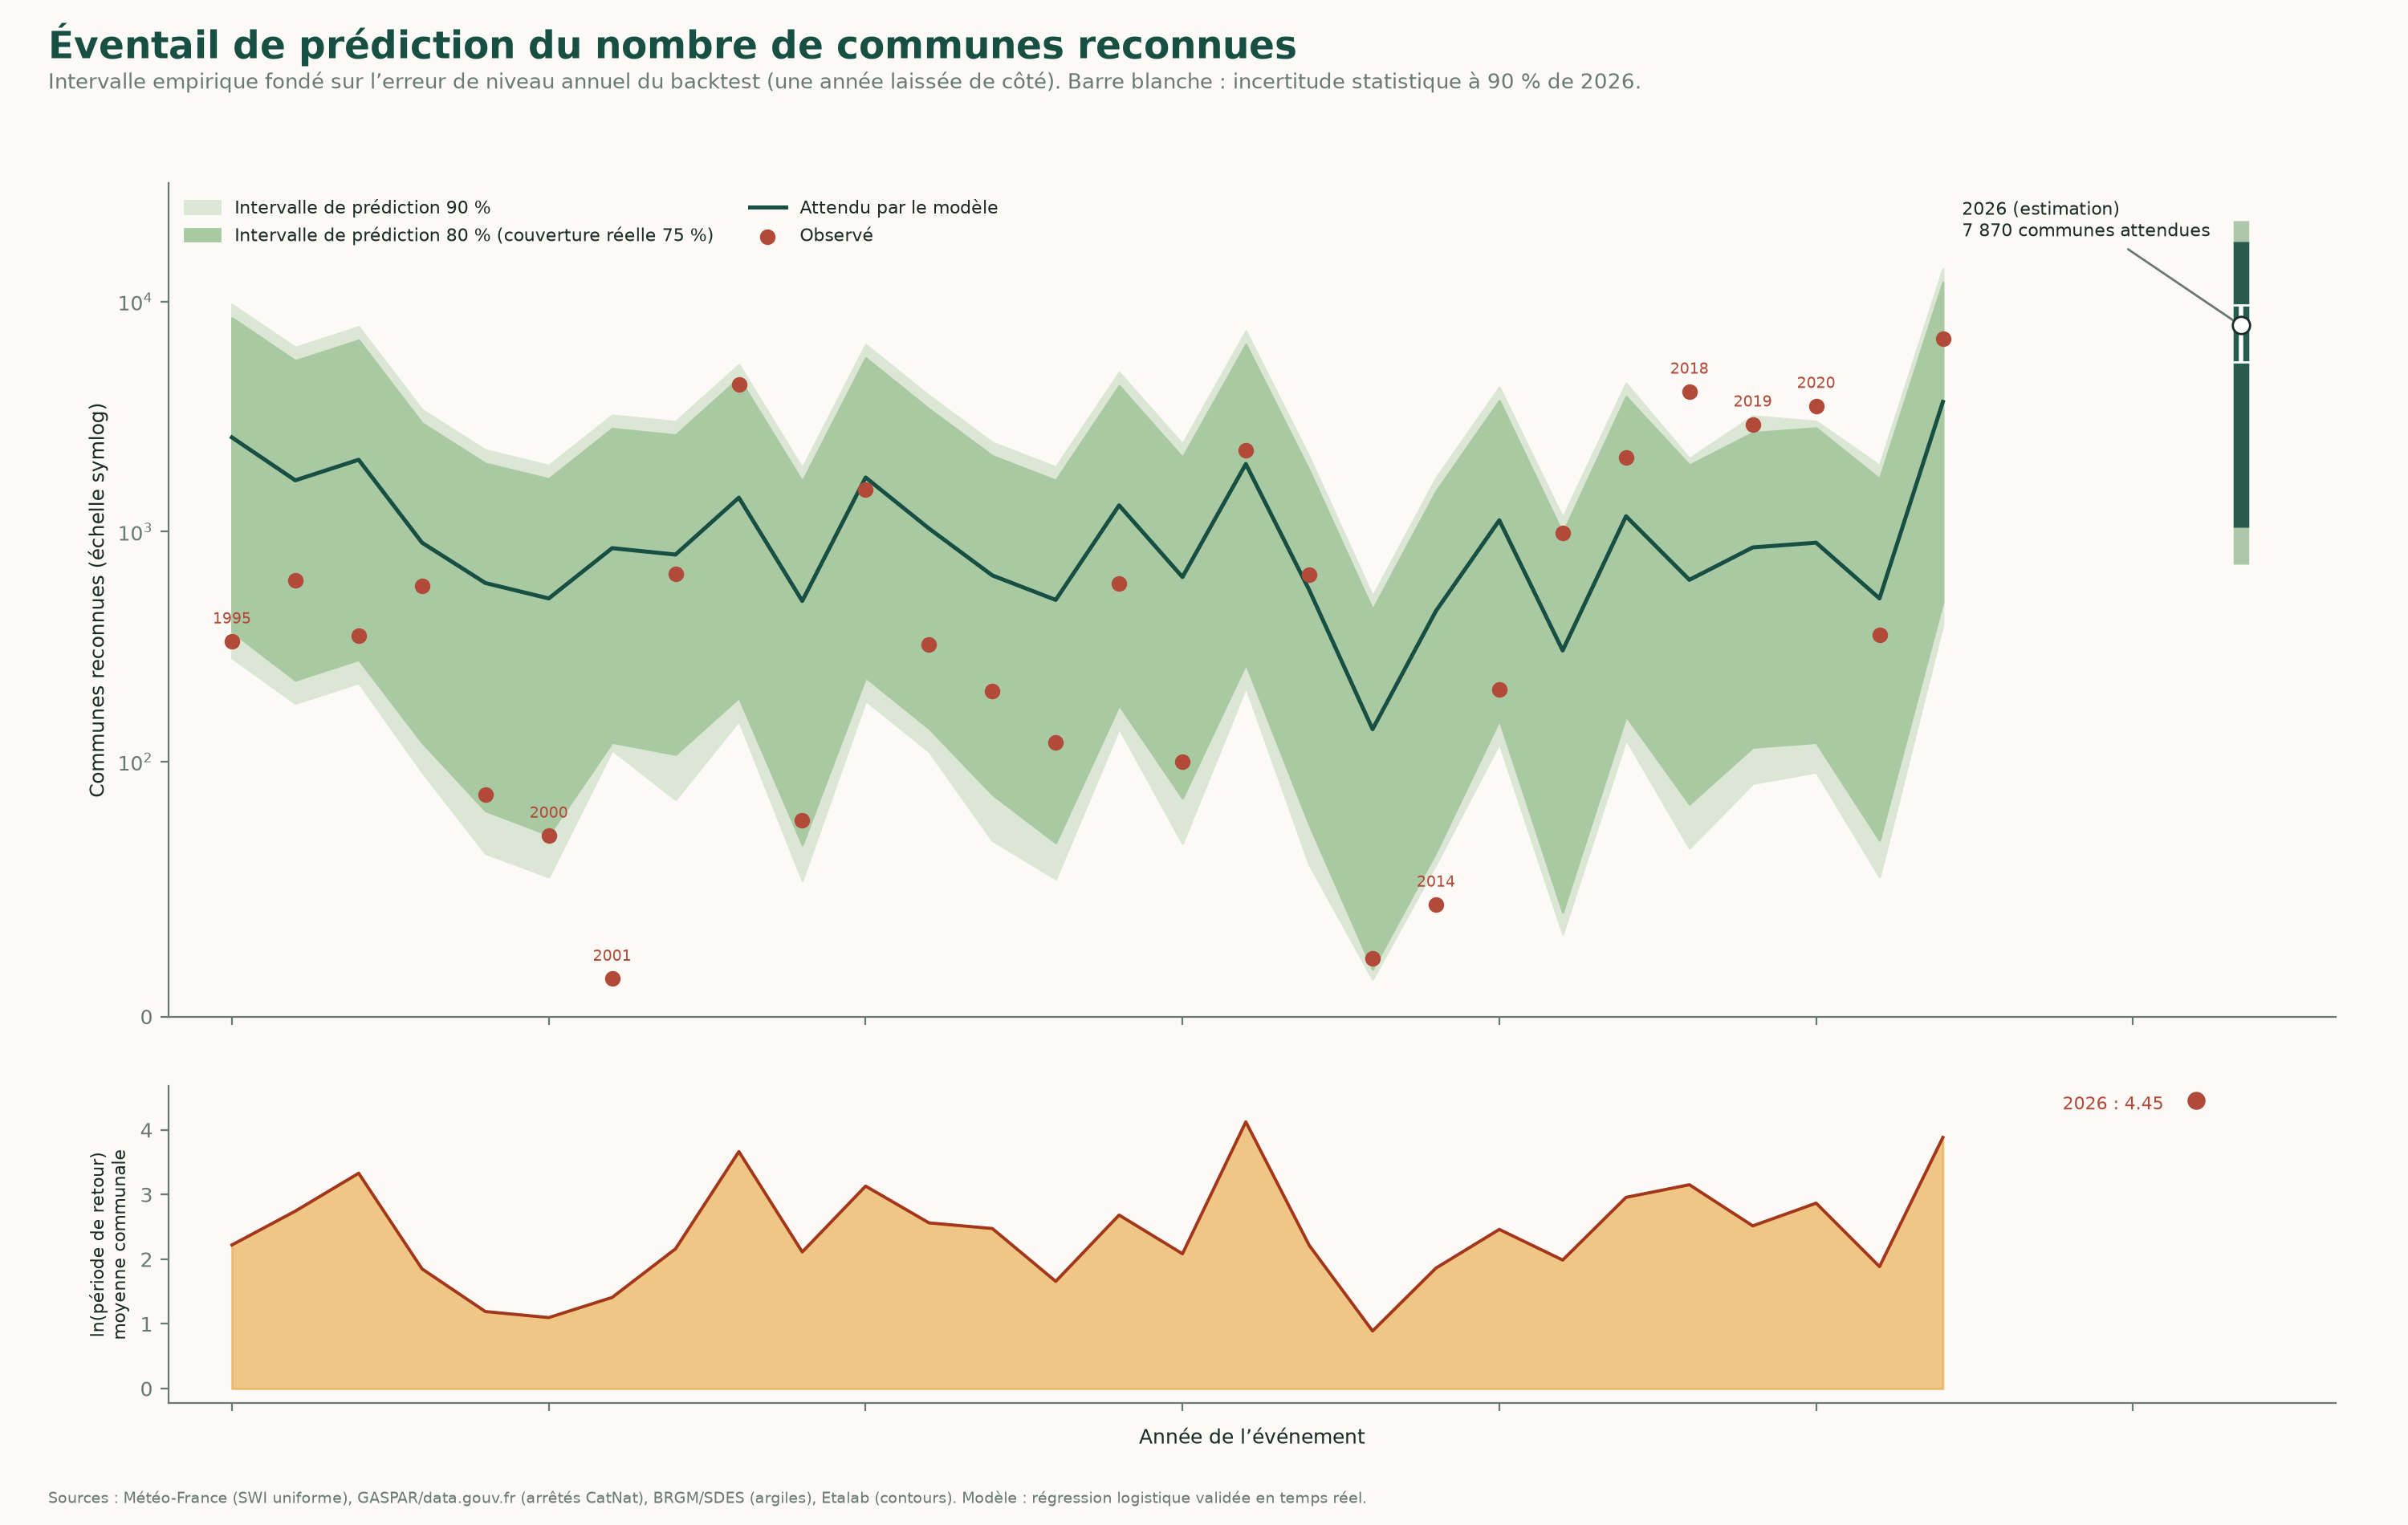
\includegraphics[width=\linewidth]{pro_eventail_prediction.png}\caption{Éventail de prédiction du nombre de communes reconnues : intervalles empiriques du backtest et estimation 2026.}\end{figure}
\begin{figure}[H]\centering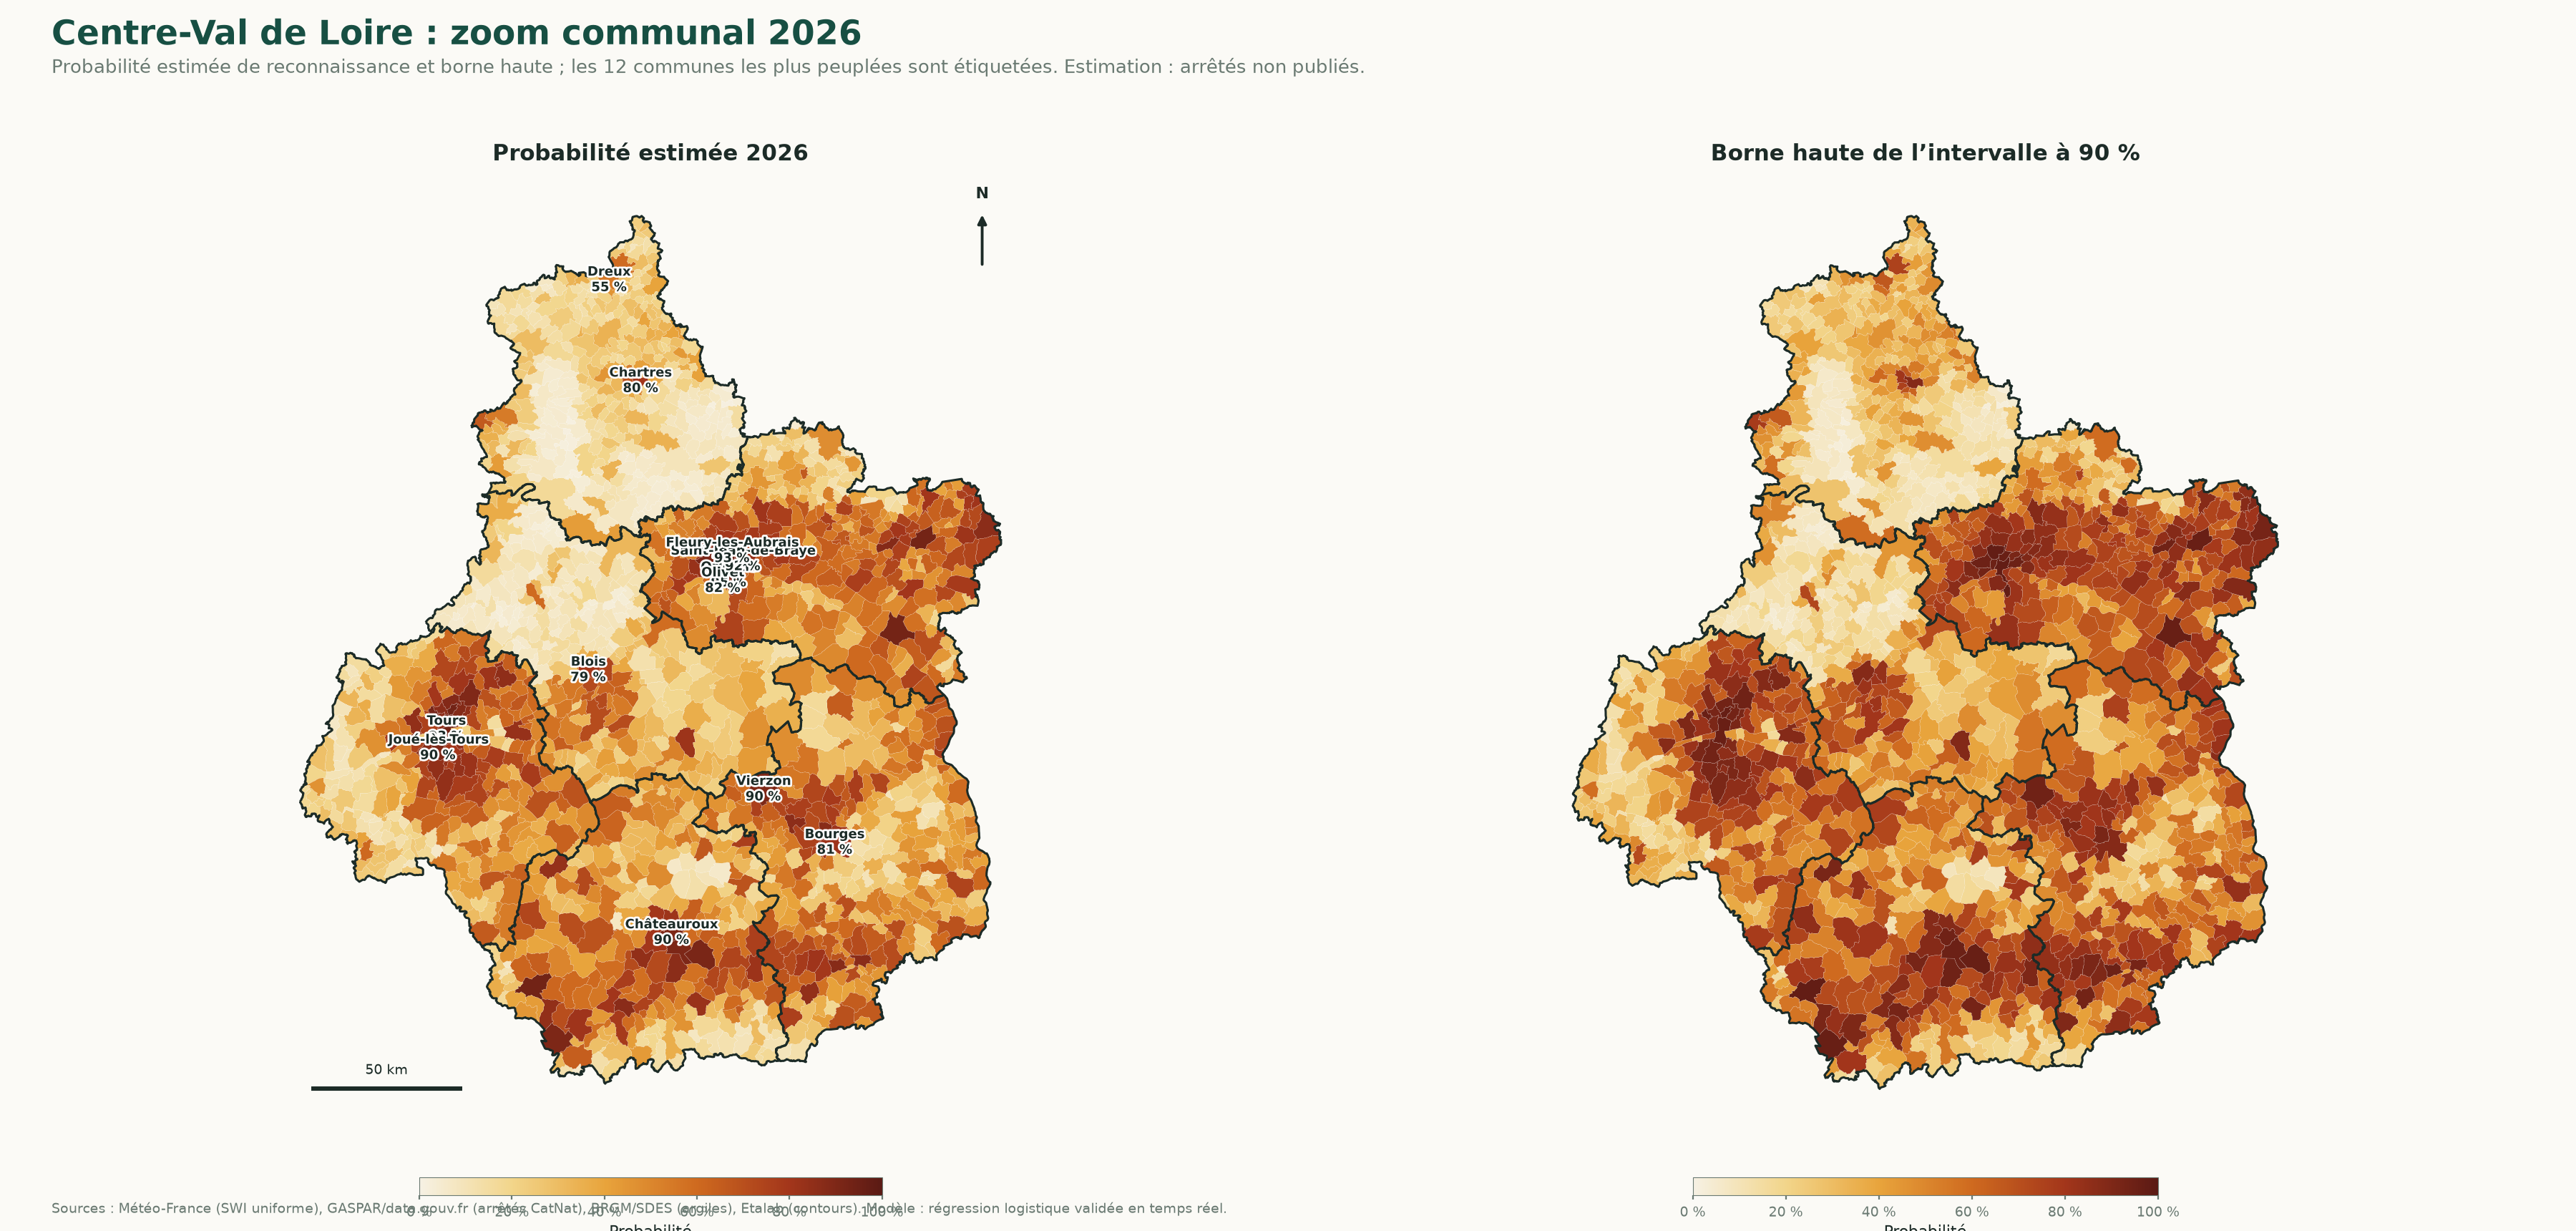
\includegraphics[width=\linewidth]{pro_region_24_2026.png}\caption{Zoom communal sur le Centre-Val de Loire.}\end{figure}
\begin{figure}[H]\centering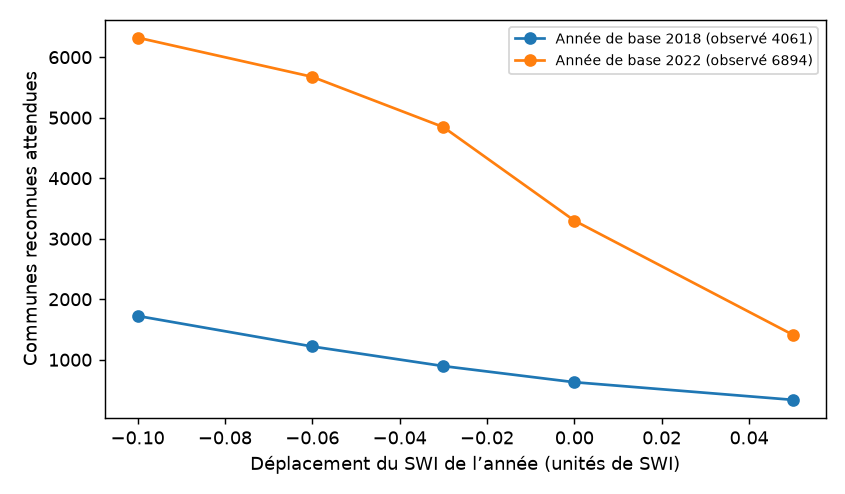
\includegraphics[width=.9\linewidth]{climate_sensibilite.png}\caption{Sensibilité du nombre attendu de communes à un déplacement du SWI.}\end{figure}

\section{Limites}
\begin{itemize}
\item \textbf{Fréquence, pas charge} : aucune donnée publique de sinistres ou de coûts à la commune ; pas de prime pure.
\item \textbf{Niveau annuel non stationnaire} : la procédure de reconnaissance a évolué ; le centre de l'intervalle de prédiction n'est pas fiable, seule l'enveloppe est utilisable. 2026 est plus sévère que toute année d'apprentissage : le modèle extrapole.
\item Le critère météorologique est une reconstitution ; l'aléa argile communal est calculé sur des contours simplifiés à 100\,m ; population et contours sont des photographies récentes.
\item Tendances et sensibilité : réanalyse et test de décalage, pas des projections climatiques.
\end{itemize}
\smallnote{Code et données : dépôt kelian19/ml-climate-risk-catnat. Résultats : reports/*.json.}
\end{document}
